\documentclass[1p]{elsarticle_modified}
%\bibliographystyle{elsarticle-num}

%\usepackage[colorlinks]{hyperref}
%\usepackage{abbrmath_seonhwa} %\Abb, \Ascr, \Acal ,\Abf, \Afrak
\usepackage{amsfonts}
\usepackage{amssymb}
\usepackage{amsmath}
\usepackage{amsthm}
\usepackage{scalefnt}
\usepackage{amsbsy}
\usepackage{kotex}
\usepackage{caption}
\usepackage{subfig}
\usepackage{color}
\usepackage{graphicx}
\usepackage{xcolor} %% white, black, red, green, blue, cyan, magenta, yellow
\usepackage{float}
\usepackage{setspace}
\usepackage{hyperref}

\usepackage{tikz}
\usetikzlibrary{arrows}

\usepackage{multirow}
\usepackage{array} % fixed length table
\usepackage{hhline}

%%%%%%%%%%%%%%%%%%%%%
\makeatletter
\renewcommand*\env@matrix[1][\arraystretch]{%
	\edef\arraystretch{#1}%
	\hskip -\arraycolsep
	\let\@ifnextchar\new@ifnextchar
	\array{*\c@MaxMatrixCols c}}
\makeatother %https://tex.stackexchange.com/questions/14071/how-can-i-increase-the-line-spacing-in-a-matrix
%%%%%%%%%%%%%%%

\usepackage[normalem]{ulem}

\newcommand{\msout}[1]{\ifmmode\text{\sout{\ensuremath{#1}}}\else\sout{#1}\fi}
%SOURCE: \msout is \stkout macro in https://tex.stackexchange.com/questions/20609/strikeout-in-math-mode

\newcommand{\cancel}[1]{
	\ifmmode
	{\color{red}\msout{#1}}
	\else
	{\color{red}\sout{#1}}
	\fi
}

\newcommand{\add}[1]{
	{\color{blue}\uwave{#1}}
}

\newcommand{\replace}[2]{
	\ifmmode
	{\color{red}\msout{#1}}{\color{blue}\uwave{#2}}
	\else
	{\color{red}\sout{#1}}{\color{blue}\uwave{#2}}
	\fi
}

\newcommand{\Sol}{\mathcal{S}} %segment
\newcommand{\D}{D} %diagram
\newcommand{\A}{\mathcal{A}} %arc


%%%%%%%%%%%%%%%%%%%%%%%%%%%%%5 test

\def\sl{\operatorname{\textup{SL}}(2,\Cbb)}
\def\psl{\operatorname{\textup{PSL}}(2,\Cbb)}
\def\quan{\mkern 1mu \triangleright \mkern 1mu}

\theoremstyle{definition}
\newtheorem{thm}{Theorem}[section]
\newtheorem{prop}[thm]{Proposition}
\newtheorem{lem}[thm]{Lemma}
\newtheorem{ques}[thm]{Question}
\newtheorem{cor}[thm]{Corollary}
\newtheorem{defn}[thm]{Definition}
\newtheorem{exam}[thm]{Example}
\newtheorem{rmk}[thm]{Remark}
\newtheorem{alg}[thm]{Algorithm}

\newcommand{\I}{\sqrt{-1}}
\begin{document}

%\begin{frontmatter}
%
%\title{Boundary parabolic representations of knots up to 8 crossings}
%
%%% Group authors per affiliation:
%\author{Yunhi Cho} 
%\address{Department of Mathematics, University of Seoul, Seoul, Korea}
%\ead{yhcho@uos.ac.kr}
%
%
%\author{Seonhwa Kim} %\fnref{s_kim}}
%\address{Center for Geometry and Physics, Institute for Basic Science, Pohang, 37673, Korea}
%\ead{ryeona17@ibs.re.kr}
%
%\author{Hyuk Kim}
%\address{Department of Mathematical Sciences, Seoul National University, Seoul 08826, Korea}
%\ead{hyukkim@snu.ac.kr}
%
%\author{Seokbeom Yoon}
%\address{Department of Mathematical Sciences, Seoul National University, Seoul, 08826,  Korea}
%\ead{sbyoon15@snu.ac.kr}
%
%\begin{abstract}
%We find all boundary parabolic representation of knots up to 8 crossings.
%
%\end{abstract}
%\begin{keyword}
%    \MSC[2010] 57M25 
%\end{keyword}
%
%\end{frontmatter}

%\linenumbers
%\tableofcontents
%
\newcommand\colored[1]{\textcolor{white}{\rule[-0.35ex]{0.8em}{1.4ex}}\kern-0.8em\color{red} #1}%
%\newcommand\colored[1]{\textcolor{white}{ #1}\kern-2.17ex	\textcolor{white}{ #1}\kern-1.81ex	\textcolor{white}{ #1}\kern-2.15ex\color{red}#1	}

{\Large $\underline{12n_{0843}~(K12n_{0843})}$}

\setlength{\tabcolsep}{10pt}
\renewcommand{\arraystretch}{1.6}
\vspace{1cm}\begin{tabular}{m{100pt}>{\centering\arraybackslash}m{274pt}}
\multirow{5}{120pt}{
	\centering
	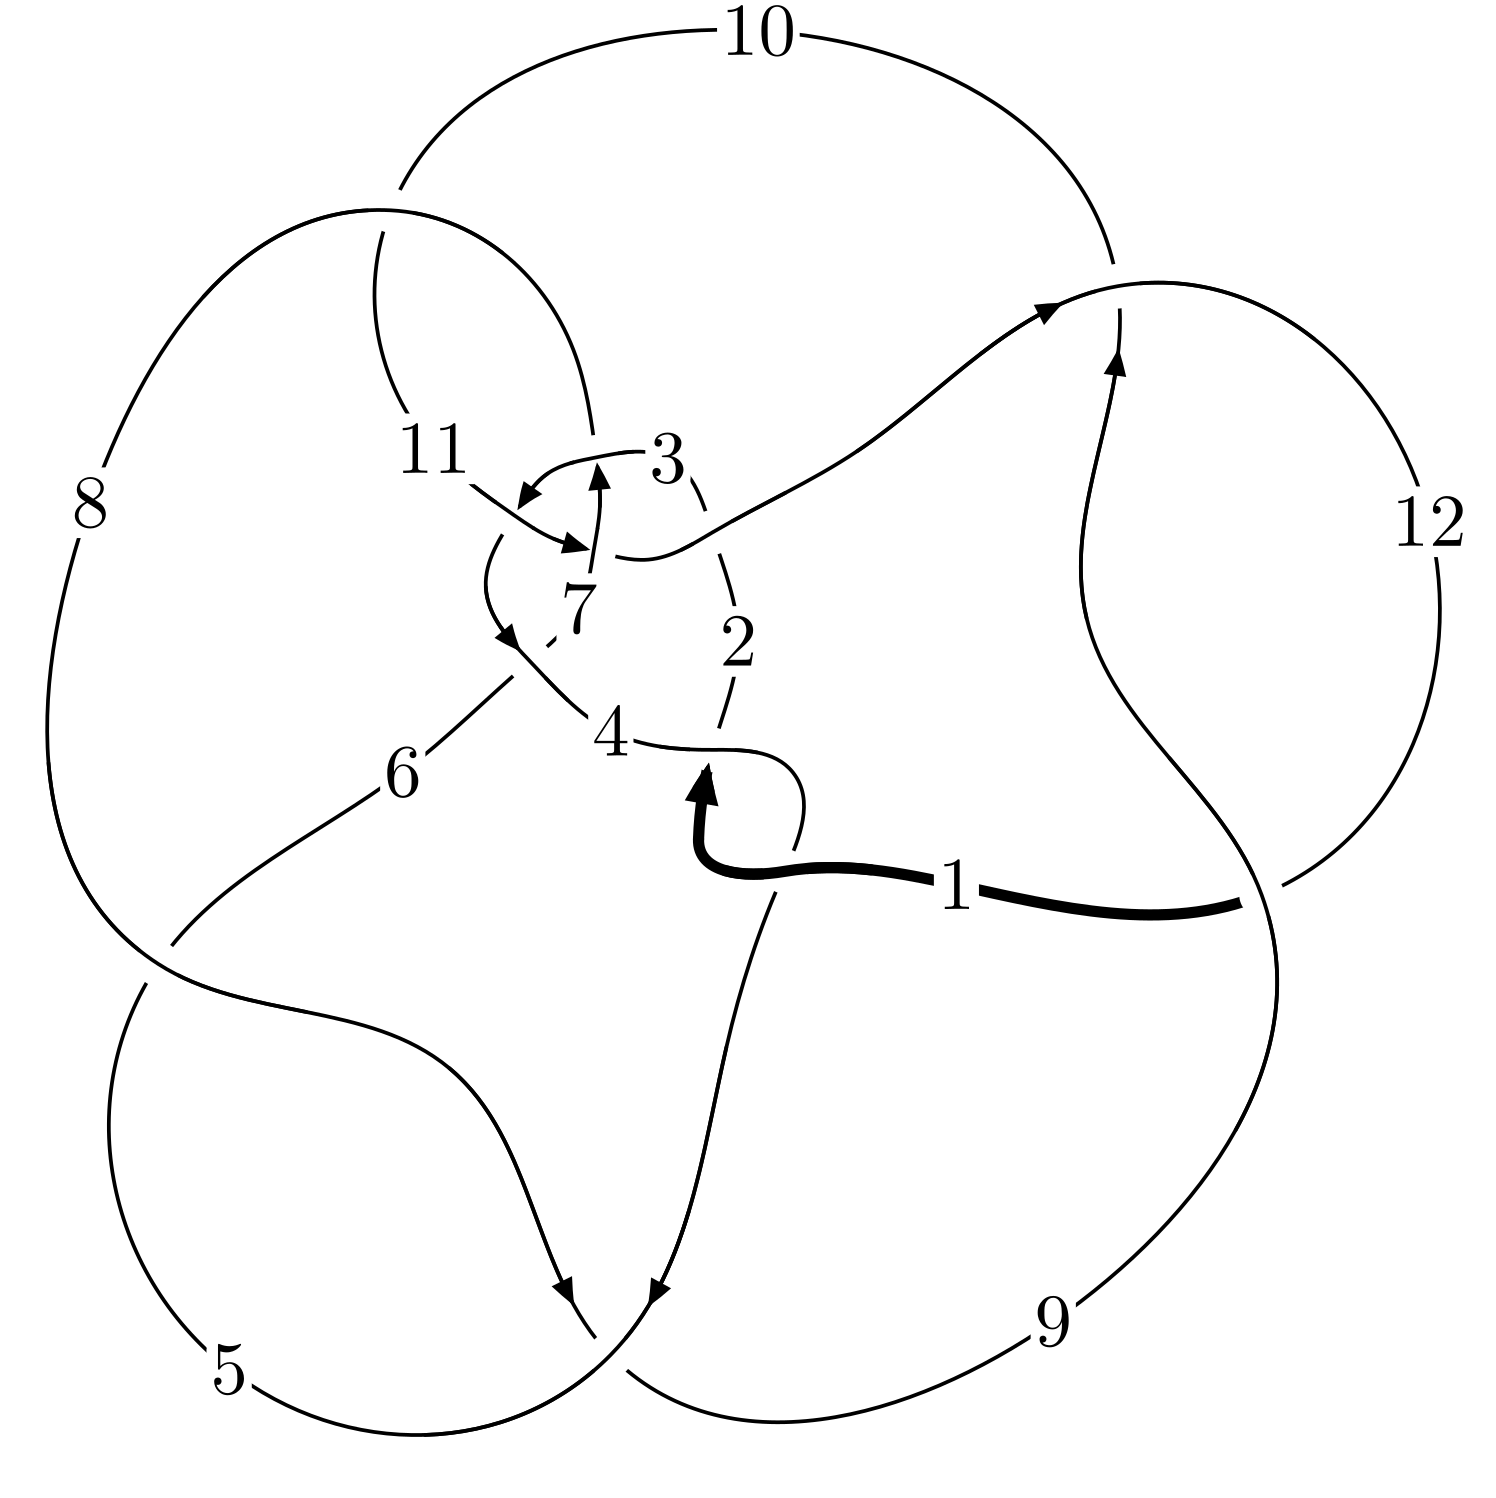
\includegraphics[width=112pt]{../../../GIT/diagram.site/Diagrams/png/2932_12n_0843.png}\\
\ \ \ A knot diagram\footnotemark}&
\allowdisplaybreaks
\textbf{Linearized knot diagam} \\
\cline{2-2}
 &
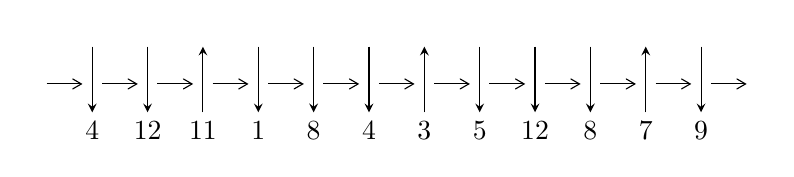
\begin{tikzpicture}[x=20pt, y=17pt]
	% nodes
	\node (C0) at (0, 0) {};
	\node (C1) at (1, 0) {};
	\node (C1U) at (1, +1) {};
	\node (C1D) at (1, -1) {4};

	\node (C2) at (2, 0) {};
	\node (C2U) at (2, +1) {};
	\node (C2D) at (2, -1) {12};

	\node (C3) at (3, 0) {};
	\node (C3U) at (3, +1) {};
	\node (C3D) at (3, -1) {11};

	\node (C4) at (4, 0) {};
	\node (C4U) at (4, +1) {};
	\node (C4D) at (4, -1) {1};

	\node (C5) at (5, 0) {};
	\node (C5U) at (5, +1) {};
	\node (C5D) at (5, -1) {8};

	\node (C6) at (6, 0) {};
	\node (C6U) at (6, +1) {};
	\node (C6D) at (6, -1) {4};

	\node (C7) at (7, 0) {};
	\node (C7U) at (7, +1) {};
	\node (C7D) at (7, -1) {3};

	\node (C8) at (8, 0) {};
	\node (C8U) at (8, +1) {};
	\node (C8D) at (8, -1) {5};

	\node (C9) at (9, 0) {};
	\node (C9U) at (9, +1) {};
	\node (C9D) at (9, -1) {12};

	\node (C10) at (10, 0) {};
	\node (C10U) at (10, +1) {};
	\node (C10D) at (10, -1) {8};

	\node (C11) at (11, 0) {};
	\node (C11U) at (11, +1) {};
	\node (C11D) at (11, -1) {7};

	\node (C12) at (12, 0) {};
	\node (C12U) at (12, +1) {};
	\node (C12D) at (12, -1) {9};
	\node (C13) at (13, 0) {};

	% arrows
	\draw[->,>={angle 60}]
	(C0) edge (C1) (C1) edge (C2) (C2) edge (C3) (C3) edge (C4) (C4) edge (C5) (C5) edge (C6) (C6) edge (C7) (C7) edge (C8) (C8) edge (C9) (C9) edge (C10) (C10) edge (C11) (C11) edge (C12) (C12) edge (C13) ;	\draw[->,>=stealth]
	(C1U) edge (C1D) (C2U) edge (C2D) (C3D) edge (C3U) (C4U) edge (C4D) (C5U) edge (C5D) (C6U) edge (C6D) (C7D) edge (C7U) (C8U) edge (C8D) (C9U) edge (C9D) (C10U) edge (C10D) (C11D) edge (C11U) (C12U) edge (C12D) ;
	\end{tikzpicture} \\
\hhline{~~} \\& 
\textbf{Solving Sequence} \\ \cline{2-2} 
 &
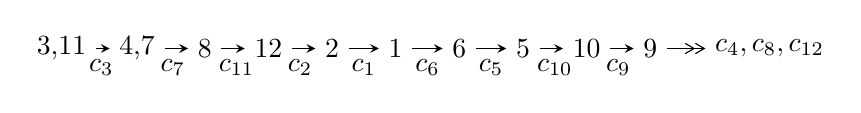
\begin{tikzpicture}[x=23pt, y=7pt]
	% node
	\node (A0) at (-1/8, 0) {3,11};
	\node (A1) at (17/16, 0) {4,7};
	\node (A2) at (17/8, 0) {8};
	\node (A3) at (25/8, 0) {12};
	\node (A4) at (33/8, 0) {2};
	\node (A5) at (41/8, 0) {1};
	\node (A6) at (49/8, 0) {6};
	\node (A7) at (57/8, 0) {5};
	\node (A8) at (65/8, 0) {10};
	\node (A9) at (73/8, 0) {9};
	\node (C1) at (1/2, -1) {$c_{3}$};
	\node (C2) at (13/8, -1) {$c_{7}$};
	\node (C3) at (21/8, -1) {$c_{11}$};
	\node (C4) at (29/8, -1) {$c_{2}$};
	\node (C5) at (37/8, -1) {$c_{1}$};
	\node (C6) at (45/8, -1) {$c_{6}$};
	\node (C7) at (53/8, -1) {$c_{5}$};
	\node (C8) at (61/8, -1) {$c_{10}$};
	\node (C9) at (69/8, -1) {$c_{9}$};
	\node (A10) at (11, 0) {$c_{4},c_{8},c_{12}$};

	% edge
	\draw[->,>=stealth]	
	(A0) edge (A1) (A1) edge (A2) (A2) edge (A3) (A3) edge (A4) (A4) edge (A5) (A5) edge (A6) (A6) edge (A7) (A7) edge (A8) (A8) edge (A9) ;
	\draw[->>,>={angle 60}]	
	(A9) edge (A10);
\end{tikzpicture} \\ 

\end{tabular} \\

\footnotetext{
The image of knot diagram is generated by the software ``\textbf{Draw programme}" developed by Andrew Bartholomew(\url{http://www.layer8.co.uk/maths/draw/index.htm\#Running-draw}), where we modified some parts for our purpose(\url{https://github.com/CATsTAILs/LinksPainter}).
}\phantom \\ \newline 
\centering \textbf{Ideals for irreducible components\footnotemark of $X_{\text{par}}$} 
 
\begin{align*}
I^u_{1}&=\langle 
b- u,\;a-1,\;u^6+3 u^5+5 u^4+4 u^3+3 u^2+2 u+1\rangle \\
I^u_{2}&=\langle 
6910924 u^{19}+111764718 u^{18}+\cdots+18467014 b+50164092,\\
\phantom{I^u_{2}}&\phantom{= \langle  }-12541023 u^{19}-199375543 u^{18}+\cdots+36934028 a-54583614,\;u^{20}+17 u^{19}+\cdots-58 u^2+8\rangle \\
I^u_{3}&=\langle 
b- u,\;201231 u^{19}-801753 u^{18}+\cdots+26914 a-196045,\;u^{20}-4 u^{19}+\cdots-4 u+1\rangle \\
I^u_{4}&=\langle 
3171 u^{19}-102100 u^{18}+\cdots+26914 b-201231,\;a-1,\;u^{20}-4 u^{19}+\cdots-4 u+1\rangle \\
I^u_{5}&=\langle 
b+u,\;a+1,\;u^8+3 u^7+4 u^6+u^5-2 u^4-2 u^3+1\rangle \\
I^u_{6}&=\langle 
-47 u^{11}-28 u^{10}+\cdots+592 b-663,\;663 u^{11} a+949 u^{11}+\cdots-913 a-2279,\\
\phantom{I^u_{6}}&\phantom{= \langle  }u^{12}-3 u^{11}+4 u^{10}+3 u^9-9 u^8+5 u^7+15 u^6-23 u^5+20 u^4-9 u^3+4 u^2- u+1\rangle \\
I^u_{7}&=\langle 
b+u,\;2 u^7-6 u^6+7 u^5-2 u^4-4 u^2+a+5 u-3,\;u^8-3 u^7+4 u^6-2 u^5+u^4-2 u^3+3 u^2-2 u+1\rangle \\
I^u_{8}&=\langle 
- u^6+2 u^5-2 u^4- u^2+b+u-2,\;a+1,\;u^8-3 u^7+4 u^6-2 u^5+u^4-2 u^3+3 u^2-2 u+1\rangle \\
I^u_{9}&=\langle 
- u^7-4 u^6-7 u^5-5 u^4+u^2+b- u,\;- u^6-4 u^5-7 u^4-5 u^3+a+u-1,\\
\phantom{I^u_{9}}&\phantom{= \langle  }u^8+5 u^7+12 u^6+16 u^5+13 u^4+7 u^3+4 u^2+2 u+1\rangle \\
I^u_{10}&=\langle 
- u^4+2 u^3-2 u^2+b+2 u-2,\;u^4-2 u^3+u^2+a+1,\;u^6-3 u^5+4 u^4-4 u^3+4 u^2-2 u+1\rangle \\
\end{align*}\\
\begin{align*}
I^u_{11}&=\langle 
u^5-2 u^4+u^3+b+u,\;2 u^5-6 u^4+7 u^3-6 u^2+a+6 u-2,\;u^6-3 u^5+4 u^4-4 u^3+4 u^2-2 u+1\rangle \\
I^u_{12}&=\langle 
b- u,\;a-1,\;u^3+u^2+u-1\rangle \\
\\
\end{align*}
\raggedright * 12 irreducible components of $\dim_{\mathbb{C}}=0$, with total 137 representations.\\
\footnotetext{All coefficients of polynomials are rational numbers. But the coefficients are sometimes approximated in decimal forms when there is not enough margin.}
\newpage
\renewcommand{\arraystretch}{1}
\centering \section*{I. $I^u_{1}= \langle b- u,\;a-1,\;u^6+3 u^5+5 u^4+4 u^3+3 u^2+2 u+1 \rangle$}
\flushleft \textbf{(i) Arc colorings}\\
\begin{tabular}{m{7pt} m{180pt} m{7pt} m{180pt} }
\flushright $a_{3}=$&$\begin{pmatrix}1\\0\end{pmatrix}$ \\
\flushright $a_{11}=$&$\begin{pmatrix}0\\u\end{pmatrix}$ \\
\flushright $a_{4}=$&$\begin{pmatrix}1\\- u^2\end{pmatrix}$ \\
\flushright $a_{7}=$&$\begin{pmatrix}1\\u\end{pmatrix}$ \\
\flushright $a_{8}=$&$\begin{pmatrix}u+1\\u\end{pmatrix}$ \\
\flushright $a_{12}=$&$\begin{pmatrix}u\\u^2+u\end{pmatrix}$ \\
\flushright $a_{2}=$&$\begin{pmatrix}- u^3- u^2+1\\- u^4-2 u^3- u^2\end{pmatrix}$ \\
\flushright $a_{1}=$&$\begin{pmatrix}- u^5-2 u^4-3 u^3- u^2+1\\- u^3+u+1\end{pmatrix}$ \\
\flushright $a_{6}=$&$\begin{pmatrix}u^2+u+1\\- u^4- u^3+u\end{pmatrix}$ \\
\flushright $a_{5}=$&$\begin{pmatrix}u^4+2 u^3+4 u^2+3 u+2\\u^5+2 u^4+3 u^3+3 u^2+3 u+1\end{pmatrix}$ \\
\flushright $a_{10}=$&$\begin{pmatrix}u^3+2 u^2+u\\u^3+u^2+u\end{pmatrix}$ \\
\flushright $a_{9}=$&$\begin{pmatrix}u^5+3 u^4+5 u^3+5 u^2+3 u+1\\u^5+2 u^4+4 u^3+3 u^2+2 u\end{pmatrix}$\\&\end{tabular}
\flushleft \textbf{(ii) Obstruction class $= -1$}\\~\\
\flushleft \textbf{(iii) Cusp Shapes $= 3 u^5+9 u^4+12 u^3+3 u^2+3 u+3$}\\~\\
\newpage\renewcommand{\arraystretch}{1}
\flushleft \textbf{(iv) u-Polynomials at the component}\newline \\
\begin{tabular}{m{50pt}|m{274pt}}
Crossings & \hspace{64pt}u-Polynomials at each crossing \\
\hline $$\begin{aligned}c_{1},c_{4},c_{5}\\c_{8},c_{9},c_{12}\end{aligned}$$&$\begin{aligned}
&u^6-2 u^5+5 u^4-4 u^3+5 u^2- u+1
\end{aligned}$\\
\hline $$\begin{aligned}c_{2},c_{6},c_{10}\end{aligned}$$&$\begin{aligned}
&u^6-4 u^5+9 u^4-11 u^3+10 u^2-5 u+1
\end{aligned}$\\
\hline $$\begin{aligned}c_{3},c_{7},c_{11}\end{aligned}$$&$\begin{aligned}
&u^6-3 u^5+5 u^4-4 u^3+3 u^2-2 u+1
\end{aligned}$\\
\hline
\end{tabular}\\~\\
\newpage\renewcommand{\arraystretch}{1}
\flushleft \textbf{(v) Riley Polynomials at the component}\newline \\
\begin{tabular}{m{50pt}|m{274pt}}
Crossings & \hspace{64pt}Riley Polynomials at each crossing \\
\hline $$\begin{aligned}c_{1},c_{4},c_{5}\\c_{8},c_{9},c_{12}\end{aligned}$$&$\begin{aligned}
&y^6+6 y^5+19 y^4+32 y^3+27 y^2+9 y+1
\end{aligned}$\\
\hline $$\begin{aligned}c_{2},c_{6},c_{10}\end{aligned}$$&$\begin{aligned}
&y^6+2 y^5+13 y^4+21 y^3+8 y^2-5 y+1
\end{aligned}$\\
\hline $$\begin{aligned}c_{3},c_{7},c_{11}\end{aligned}$$&$\begin{aligned}
&y^6+y^5+7 y^4+4 y^3+3 y^2+2 y+1
\end{aligned}$\\
\hline
\end{tabular}\\~\\
\newpage\flushleft \textbf{(vi) Complex Volumes and Cusp Shapes}
$$\begin{array}{c|c|c}  
\text{Solutions to }I^u_{1}& \I (\text{vol} + \sqrt{-1}CS) & \text{Cusp shape}\\
 \hline 
\begin{aligned}
u &= -0.662897 + 0.491150 I \\
a &= \phantom{-}1.00000\phantom{ +0.000000I} \\
b &= -0.662897 + 0.491150 I\end{aligned}
 & \phantom{-}0.95398 - 1.33057 I & \phantom{-}1.54996 + 3.49130 I \\ \hline\begin{aligned}
u &= -0.662897 - 0.491150 I \\
a &= \phantom{-}1.00000\phantom{ +0.000000I} \\
b &= -0.662897 - 0.491150 I\end{aligned}
 & \phantom{-}0.95398 + 1.33057 I & \phantom{-}1.54996 - 3.49130 I \\ \hline\begin{aligned}
u &= \phantom{-}0.233407 + 0.727795 I \\
a &= \phantom{-}1.00000\phantom{ +0.000000I} \\
b &= \phantom{-}0.233407 + 0.727795 I\end{aligned}
 & \phantom{-}5.70894 + 1.27621 I & -0.24770 - 2.88719 I \\ \hline\begin{aligned}
u &= \phantom{-}0.233407 - 0.727795 I \\
a &= \phantom{-}1.00000\phantom{ +0.000000I} \\
b &= \phantom{-}0.233407 - 0.727795 I\end{aligned}
 & \phantom{-}5.70894 - 1.27621 I & -0.24770 + 2.88719 I \\ \hline\begin{aligned}
u &= -1.07051 + 1.17004 I \\
a &= \phantom{-}1.00000\phantom{ +0.000000I} \\
b &= -1.07051 + 1.17004 I\end{aligned}
 & \phantom{-}1.5618 - 18.5814 I & -2.80226 + 9.65875 I \\ \hline\begin{aligned}
u &= -1.07051 - 1.17004 I \\
a &= \phantom{-}1.00000\phantom{ +0.000000I} \\
b &= -1.07051 - 1.17004 I\end{aligned}
 & \phantom{-}1.5618 + 18.5814 I & -2.80226 - 9.65875 I\\
 \hline 
 \end{array}$$\newpage\newpage\renewcommand{\arraystretch}{1}
\centering \section*{II. $I^u_{2}= \langle 6.91\times10^{6} u^{19}+1.12\times10^{8} u^{18}+\cdots+1.85\times10^{7} b+5.02\times10^{7},\;-1.25\times10^{7} u^{19}-1.99\times10^{8} u^{18}+\cdots+3.69\times10^{7} a-5.46\times10^{7},\;u^{20}+17 u^{19}+\cdots-58 u^2+8 \rangle$}
\flushleft \textbf{(i) Arc colorings}\\
\begin{tabular}{m{7pt} m{180pt} m{7pt} m{180pt} }
\flushright $a_{3}=$&$\begin{pmatrix}1\\0\end{pmatrix}$ \\
\flushright $a_{11}=$&$\begin{pmatrix}0\\u\end{pmatrix}$ \\
\flushright $a_{4}=$&$\begin{pmatrix}1\\- u^2\end{pmatrix}$ \\
\flushright $a_{7}=$&$\begin{pmatrix}0.339552 u^{19}+5.39815 u^{18}+\cdots+7.20308 u+1.47787\\-0.374231 u^{19}-6.05213 u^{18}+\cdots+1.47787 u-2.71642\end{pmatrix}$ \\
\flushright $a_{8}=$&$\begin{pmatrix}-0.0346787 u^{19}-0.653974 u^{18}+\cdots+8.68095 u-1.23855\\-0.374231 u^{19}-6.05213 u^{18}+\cdots+1.47787 u-2.71642\end{pmatrix}$ \\
\flushright $a_{12}=$&$\begin{pmatrix}0.692665 u^{19}+11.3252 u^{18}+\cdots-16.9750 u+4.33805\\-0.450082 u^{19}-7.21967 u^{18}+\cdots+5.33805 u-5.54132\end{pmatrix}$ \\
\flushright $a_{2}=$&$\begin{pmatrix}-0.0222967 u^{19}-0.221327 u^{18}+\cdots-4.64076 u-3.18001\\-0.274012 u^{19}-4.37474 u^{18}+\cdots+1.36131 u-3.42229\end{pmatrix}$ \\
\flushright $a_{1}=$&$\begin{pmatrix}-0.601980 u^{19}-9.66925 u^{18}+\cdots-3.10107 u-7.86403\\-0.161223 u^{19}-2.34621 u^{18}+\cdots-3.27616 u-0.168684\end{pmatrix}$ \\
\flushright $a_{6}=$&$\begin{pmatrix}0.275116 u^{19}+4.43129 u^{18}+\cdots+5.96453 u+1.75530\\-0.359034 u^{19}-5.59838 u^{18}+\cdots+0.962383 u-1.68803\end{pmatrix}$ \\
\flushright $a_{5}=$&$\begin{pmatrix}0.721282 u^{19}+11.6179 u^{18}+\cdots+1.13408 u+1.99349\\-1.07481 u^{19}-17.4491 u^{18}+\cdots+10.4961 u-10.9836\end{pmatrix}$ \\
\flushright $a_{10}=$&$\begin{pmatrix}0.224229 u^{19}+3.63613 u^{18}+\cdots-13.8402 u-3.14393\\-0.0183541 u^{19}-0.469426 u^{18}+\cdots-0.203268 u-1.94066\end{pmatrix}$ \\
\flushright $a_{9}=$&$\begin{pmatrix}1.19321 u^{19}+19.7559 u^{18}+\cdots-15.6737 u+8.67976\\0.0354594 u^{19}+0.212840 u^{18}+\cdots+6.93641 u-5.05504\end{pmatrix}$\\&\end{tabular}
\flushleft \textbf{(ii) Obstruction class $= -1$}\\~\\
\flushleft \textbf{(iii) Cusp Shapes $= -\frac{26183957}{18467014} u^{19}-\frac{212046660}{9233507} u^{18}+\cdots+\frac{52565092}{9233507} u-\frac{114548582}{9233507}$}\\~\\
\newpage\renewcommand{\arraystretch}{1}
\flushleft \textbf{(iv) u-Polynomials at the component}\newline \\
\begin{tabular}{m{50pt}|m{274pt}}
Crossings & \hspace{64pt}u-Polynomials at each crossing \\
\hline $$\begin{aligned}c_{1},c_{4},c_{9}\\c_{12}\end{aligned}$$&$\begin{aligned}
&u^{20}+4 u^{19}+\cdots+6 u+1
\end{aligned}$\\
\hline $$\begin{aligned}c_{2}\end{aligned}$$&$\begin{aligned}
&u^{20}-21 u^{19}+\cdots-5888 u+512
\end{aligned}$\\
\hline $$\begin{aligned}c_{3}\end{aligned}$$&$\begin{aligned}
&u^{20}-17 u^{19}+\cdots-58 u^2+8
\end{aligned}$\\
\hline $$\begin{aligned}c_{5},c_{8}\end{aligned}$$&$\begin{aligned}
&u^{20}-10 u^{19}+\cdots-432 u+64
\end{aligned}$\\
\hline $$\begin{aligned}c_{6},c_{10}\end{aligned}$$&$\begin{aligned}
&u^{20}+4 u^{19}+\cdots+9 u+1
\end{aligned}$\\
\hline $$\begin{aligned}c_{7},c_{11}\end{aligned}$$&$\begin{aligned}
&u^{20}+4 u^{19}+\cdots+4 u+1
\end{aligned}$\\
\hline
\end{tabular}\\~\\
\newpage\renewcommand{\arraystretch}{1}
\flushleft \textbf{(v) Riley Polynomials at the component}\newline \\
\begin{tabular}{m{50pt}|m{274pt}}
Crossings & \hspace{64pt}Riley Polynomials at each crossing \\
\hline $$\begin{aligned}c_{1},c_{4},c_{9}\\c_{12}\end{aligned}$$&$\begin{aligned}
&y^{20}+14 y^{19}+\cdots+18 y+1
\end{aligned}$\\
\hline $$\begin{aligned}c_{2}\end{aligned}$$&$\begin{aligned}
&y^{20}- y^{19}+\cdots+8454144 y+262144
\end{aligned}$\\
\hline $$\begin{aligned}c_{3}\end{aligned}$$&$\begin{aligned}
&y^{20}-3 y^{19}+\cdots-928 y+64
\end{aligned}$\\
\hline $$\begin{aligned}c_{5},c_{8}\end{aligned}$$&$\begin{aligned}
&y^{20}+6 y^{19}+\cdots-256 y+4096
\end{aligned}$\\
\hline $$\begin{aligned}c_{6},c_{10}\end{aligned}$$&$\begin{aligned}
&y^{20}-8 y^{19}+\cdots-29 y+1
\end{aligned}$\\
\hline $$\begin{aligned}c_{7},c_{11}\end{aligned}$$&$\begin{aligned}
&y^{20}+4 y^{19}+\cdots+10 y+1
\end{aligned}$\\
\hline
\end{tabular}\\~\\
\newpage\flushleft \textbf{(vi) Complex Volumes and Cusp Shapes}
$$\begin{array}{c|c|c}  
\text{Solutions to }I^u_{2}& \I (\text{vol} + \sqrt{-1}CS) & \text{Cusp shape}\\
 \hline 
\begin{aligned}
u &= -0.591919 + 0.779585 I \\
a &= \phantom{-}1.47738 + 0.32947 I \\
b &= -1.13134 + 0.95673 I\end{aligned}
 & \phantom{-}5.94853 - 3.83843 I & -3.28174 + 4.00815 I \\ \hline\begin{aligned}
u &= -0.591919 - 0.779585 I \\
a &= \phantom{-}1.47738 - 0.32947 I \\
b &= -1.13134 - 0.95673 I\end{aligned}
 & \phantom{-}5.94853 + 3.83843 I & -3.28174 - 4.00815 I \\ \hline\begin{aligned}
u &= -0.824428 + 0.175693 I \\
a &= -1.38094 + 0.73565 I \\
b &= \phantom{-}1.009240 - 0.849113 I\end{aligned}
 & \phantom{-}7.45841 - 1.00347 I & \phantom{-}0.36457 - 2.52329 I \\ \hline\begin{aligned}
u &= -0.824428 - 0.175693 I \\
a &= -1.38094 - 0.73565 I \\
b &= \phantom{-}1.009240 + 0.849113 I\end{aligned}
 & \phantom{-}7.45841 + 1.00347 I & \phantom{-}0.36457 + 2.52329 I \\ \hline\begin{aligned}
u &= \phantom{-}0.193762 + 0.533092 I \\
a &= -0.90006 - 1.24975 I \\
b &= \phantom{-}0.491834 - 0.721967 I\end{aligned}
 & -1.94038 + 0.72654 I & -7.43882 + 4.55749 I \\ \hline\begin{aligned}
u &= \phantom{-}0.193762 - 0.533092 I \\
a &= -0.90006 + 1.24975 I \\
b &= \phantom{-}0.491834 + 0.721967 I\end{aligned}
 & -1.94038 - 0.72654 I & -7.43882 - 4.55749 I \\ \hline\begin{aligned}
u &= -0.86298 + 1.15143 I \\
a &= -1.069020 - 0.121423 I \\
b &= \phantom{-}1.06235 - 1.12612 I\end{aligned}
 & -2.00404 - 10.90100 I & -3.44699 + 8.30760 I \\ \hline\begin{aligned}
u &= -0.86298 - 1.15143 I \\
a &= -1.069020 + 0.121423 I \\
b &= \phantom{-}1.06235 + 1.12612 I\end{aligned}
 & -2.00404 + 10.90100 I & -3.44699 - 8.30760 I \\ \hline\begin{aligned}
u &= -1.01532 + 1.20528 I \\
a &= -0.852629 + 0.003707 I \\
b &= \phantom{-}0.861225 - 1.031420 I\end{aligned}
 & -3.04305 - 6.67086 I & -5.21791 + 2.63870 I \\ \hline\begin{aligned}
u &= -1.01532 - 1.20528 I \\
a &= -0.852629 - 0.003707 I \\
b &= \phantom{-}0.861225 + 1.031420 I\end{aligned}
 & -3.04305 + 6.67086 I & -5.21791 - 2.63870 I\\
 \hline 
 \end{array}$$\newpage$$\begin{array}{c|c|c}  
\text{Solutions to }I^u_{2}& \I (\text{vol} + \sqrt{-1}CS) & \text{Cusp shape}\\
 \hline 
\begin{aligned}
u &= -1.51357 + 0.59051 I \\
a &= \phantom{-}0.228246 + 0.440024 I \\
b &= -0.605304 - 0.531225 I\end{aligned}
 & -0.09983 + 3.38858 I & -2.41701 - 8.48871 I \\ \hline\begin{aligned}
u &= -1.51357 - 0.59051 I \\
a &= \phantom{-}0.228246 - 0.440024 I \\
b &= -0.605304 + 0.531225 I\end{aligned}
 & -0.09983 - 3.38858 I & -2.41701 + 8.48871 I \\ \hline\begin{aligned}
u &= \phantom{-}0.198279 + 0.120648 I \\
a &= \phantom{-}1.30829 + 4.75906 I \\
b &= -0.314766 + 1.101470 I\end{aligned}
 & \phantom{-}3.52200 - 3.40437 I & -3.46913 + 3.36431 I \\ \hline\begin{aligned}
u &= \phantom{-}0.198279 - 0.120648 I \\
a &= \phantom{-}1.30829 - 4.75906 I \\
b &= -0.314766 - 1.101470 I\end{aligned}
 & \phantom{-}3.52200 + 3.40437 I & -3.46913 - 3.36431 I \\ \hline\begin{aligned}
u &= -1.53446 + 1.05621 I \\
a &= \phantom{-}0.254710 - 0.346615 I \\
b &= -0.024746 + 0.800894 I\end{aligned}
 & \phantom{-}0.49272 - 7.72234 I & -10.36662 + 6.86541 I \\ \hline\begin{aligned}
u &= -1.53446 - 1.05621 I \\
a &= \phantom{-}0.254710 + 0.346615 I \\
b &= -0.024746 - 0.800894 I\end{aligned}
 & \phantom{-}0.49272 + 7.72234 I & -10.36662 - 6.86541 I \\ \hline\begin{aligned}
u &= -1.01845 + 1.57478 I \\
a &= -0.288306 + 0.080384 I \\
b &= \phantom{-}0.167038 - 0.535886 I\end{aligned}
 & -2.57404 - 2.62147 I & -15.2857 + 10.0855 I \\ \hline\begin{aligned}
u &= -1.01845 - 1.57478 I \\
a &= -0.288306 - 0.080384 I \\
b &= \phantom{-}0.167038 + 0.535886 I\end{aligned}
 & -2.57404 + 2.62147 I & -15.2857 - 10.0855 I \\ \hline\begin{aligned}
u &= -1.53091 + 1.32244 I \\
a &= -0.027667 - 0.334313 I \\
b &= \phantom{-}0.484465 + 0.475215 I\end{aligned}
 & \phantom{-}2.10928 + 9.64745 I & -6.0000 - 14.3164 I \\ \hline\begin{aligned}
u &= -1.53091 - 1.32244 I \\
a &= -0.027667 + 0.334313 I \\
b &= \phantom{-}0.484465 - 0.475215 I\end{aligned}
 & \phantom{-}2.10928 - 9.64745 I & -6.0000 + 14.3164 I\\
 \hline 
 \end{array}$$\newpage\newpage\renewcommand{\arraystretch}{1}
\centering \section*{III. $I^u_{3}= \langle b- u,\;2.01\times10^{5} u^{19}-8.02\times10^{5} u^{18}+\cdots+2.69\times10^{4} a-1.96\times10^{5},\;u^{20}-4 u^{19}+\cdots-4 u+1 \rangle$}
\flushleft \textbf{(i) Arc colorings}\\
\begin{tabular}{m{7pt} m{180pt} m{7pt} m{180pt} }
\flushright $a_{3}=$&$\begin{pmatrix}1\\0\end{pmatrix}$ \\
\flushright $a_{11}=$&$\begin{pmatrix}0\\u\end{pmatrix}$ \\
\flushright $a_{4}=$&$\begin{pmatrix}1\\- u^2\end{pmatrix}$ \\
\flushright $a_{7}=$&$\begin{pmatrix}-7.47682 u^{19}+29.7894 u^{18}+\cdots-36.6305 u+7.28413\\u\end{pmatrix}$ \\
\flushright $a_{8}=$&$\begin{pmatrix}-7.47682 u^{19}+29.7894 u^{18}+\cdots-35.6305 u+7.28413\\u\end{pmatrix}$ \\
\flushright $a_{12}=$&$\begin{pmatrix}17.3713 u^{19}-71.0832 u^{18}+\cdots+123.789 u-31.5849\\3.32229 u^{19}-11.0375 u^{18}+\cdots+8.00554 u+0.117820\end{pmatrix}$ \\
\flushright $a_{2}=$&$\begin{pmatrix}1.59423 u^{19}-2.41343 u^{18}+\cdots-10.6391 u-1.01835\\-1.44965 u^{19}+5.33845 u^{18}+\cdots-2.84978 u+0.253994\end{pmatrix}$ \\
\flushright $a_{1}=$&$\begin{pmatrix}2.19796 u^{19}-6.68247 u^{18}+\cdots+0.770751 u-4.72784\\0.505759 u^{19}-2.02586 u^{18}+\cdots+5.17032 u-1.60010\end{pmatrix}$ \\
\flushright $a_{6}=$&$\begin{pmatrix}-4.15453 u^{19}+18.7520 u^{18}+\cdots-28.6249 u+7.40195\\-0.502415 u^{19}+2.36568 u^{18}+\cdots-4.68433 u+2.25165\end{pmatrix}$ \\
\flushright $a_{5}=$&$\begin{pmatrix}6.35220 u^{19}-16.2202 u^{18}+\cdots-3.98086 u+4.50119\\-0.391989 u^{19}+3.27629 u^{18}+\cdots-8.30244 u+3.34528\end{pmatrix}$ \\
\flushright $a_{10}=$&$\begin{pmatrix}24.0158 u^{19}-93.1582 u^{18}+\cdots+137.800 u-31.3493\\3.32229 u^{19}-11.0375 u^{18}+\cdots+8.00554 u+0.117820\end{pmatrix}$ \\
\flushright $a_{9}=$&$\begin{pmatrix}-0.498439 u^{19}-6.37475 u^{18}+\cdots+38.7268 u-18.0626\\3.19473 u^{19}-11.9776 u^{18}+\cdots+16.8010 u-4.49101\end{pmatrix}$\\&\end{tabular}
\flushleft \textbf{(ii) Obstruction class $= -1$}\\~\\
\flushleft \textbf{(iii) Cusp Shapes $= -\frac{182014}{13457} u^{19}+\frac{673876}{13457} u^{18}+\cdots-\frac{1440624}{13457} u+\frac{66848}{13457}$}\\~\\
\newpage\renewcommand{\arraystretch}{1}
\flushleft \textbf{(iv) u-Polynomials at the component}\newline \\
\begin{tabular}{m{50pt}|m{274pt}}
Crossings & \hspace{64pt}u-Polynomials at each crossing \\
\hline $$\begin{aligned}c_{1},c_{4}\end{aligned}$$&$\begin{aligned}
&u^{20}-10 u^{19}+\cdots-432 u+64
\end{aligned}$\\
\hline $$\begin{aligned}c_{2},c_{6}\end{aligned}$$&$\begin{aligned}
&u^{20}+4 u^{19}+\cdots+9 u+1
\end{aligned}$\\
\hline $$\begin{aligned}c_{3},c_{7}\end{aligned}$$&$\begin{aligned}
&u^{20}+4 u^{19}+\cdots+4 u+1
\end{aligned}$\\
\hline $$\begin{aligned}c_{5},c_{8},c_{9}\\c_{12}\end{aligned}$$&$\begin{aligned}
&u^{20}+4 u^{19}+\cdots+6 u+1
\end{aligned}$\\
\hline $$\begin{aligned}c_{10}\end{aligned}$$&$\begin{aligned}
&u^{20}-21 u^{19}+\cdots-5888 u+512
\end{aligned}$\\
\hline $$\begin{aligned}c_{11}\end{aligned}$$&$\begin{aligned}
&u^{20}-17 u^{19}+\cdots-58 u^2+8
\end{aligned}$\\
\hline
\end{tabular}\\~\\
\newpage\renewcommand{\arraystretch}{1}
\flushleft \textbf{(v) Riley Polynomials at the component}\newline \\
\begin{tabular}{m{50pt}|m{274pt}}
Crossings & \hspace{64pt}Riley Polynomials at each crossing \\
\hline $$\begin{aligned}c_{1},c_{4}\end{aligned}$$&$\begin{aligned}
&y^{20}+6 y^{19}+\cdots-256 y+4096
\end{aligned}$\\
\hline $$\begin{aligned}c_{2},c_{6}\end{aligned}$$&$\begin{aligned}
&y^{20}-8 y^{19}+\cdots-29 y+1
\end{aligned}$\\
\hline $$\begin{aligned}c_{3},c_{7}\end{aligned}$$&$\begin{aligned}
&y^{20}+4 y^{19}+\cdots+10 y+1
\end{aligned}$\\
\hline $$\begin{aligned}c_{5},c_{8},c_{9}\\c_{12}\end{aligned}$$&$\begin{aligned}
&y^{20}+14 y^{19}+\cdots+18 y+1
\end{aligned}$\\
\hline $$\begin{aligned}c_{10}\end{aligned}$$&$\begin{aligned}
&y^{20}- y^{19}+\cdots+8454144 y+262144
\end{aligned}$\\
\hline $$\begin{aligned}c_{11}\end{aligned}$$&$\begin{aligned}
&y^{20}-3 y^{19}+\cdots-928 y+64
\end{aligned}$\\
\hline
\end{tabular}\\~\\
\newpage\flushleft \textbf{(vi) Complex Volumes and Cusp Shapes}
$$\begin{array}{c|c|c}  
\text{Solutions to }I^u_{3}& \I (\text{vol} + \sqrt{-1}CS) & \text{Cusp shape}\\
 \hline 
\begin{aligned}
u &= \phantom{-}0.491834 + 0.721967 I \\
a &= -0.379455 - 0.526881 I \\
b &= \phantom{-}0.491834 + 0.721967 I\end{aligned}
 & -1.94038 - 0.72654 I & -7.43882 - 4.55749 I \\ \hline\begin{aligned}
u &= \phantom{-}0.491834 - 0.721967 I \\
a &= -0.379455 + 0.526881 I \\
b &= \phantom{-}0.491834 - 0.721967 I\end{aligned}
 & -1.94038 + 0.72654 I & -7.43882 + 4.55749 I \\ \hline\begin{aligned}
u &= -0.314766 + 1.101470 I \\
a &= \phantom{-}0.053706 - 0.195362 I \\
b &= -0.314766 + 1.101470 I\end{aligned}
 & \phantom{-}3.52200 - 3.40437 I & -3.46913 + 3.36431 I \\ \hline\begin{aligned}
u &= -0.314766 - 1.101470 I \\
a &= \phantom{-}0.053706 + 0.195362 I \\
b &= -0.314766 - 1.101470 I\end{aligned}
 & \phantom{-}3.52200 + 3.40437 I & -3.46913 - 3.36431 I \\ \hline\begin{aligned}
u &= -0.605304 + 0.531225 I \\
a &= \phantom{-}0.92890 + 1.79077 I \\
b &= -0.605304 + 0.531225 I\end{aligned}
 & -0.09983 - 3.38858 I & -2.41701 + 8.48871 I \\ \hline\begin{aligned}
u &= -0.605304 - 0.531225 I \\
a &= \phantom{-}0.92890 - 1.79077 I \\
b &= -0.605304 - 0.531225 I\end{aligned}
 & -0.09983 + 3.38858 I & -2.41701 - 8.48871 I \\ \hline\begin{aligned}
u &= -0.024746 + 0.800894 I \\
a &= \phantom{-}1.37667 + 1.87340 I \\
b &= -0.024746 + 0.800894 I\end{aligned}
 & \phantom{-}0.49272 - 7.72234 I & -10.36662 + 6.86541 I \\ \hline\begin{aligned}
u &= -0.024746 - 0.800894 I \\
a &= \phantom{-}1.37667 - 1.87340 I \\
b &= -0.024746 - 0.800894 I\end{aligned}
 & \phantom{-}0.49272 + 7.72234 I & -10.36662 - 6.86541 I \\ \hline\begin{aligned}
u &= \phantom{-}1.009240 + 0.849113 I \\
a &= -0.564068 + 0.300488 I \\
b &= \phantom{-}1.009240 + 0.849113 I\end{aligned}
 & \phantom{-}7.45841 + 1.00347 I & \phantom{-}0.36457 + 2.52329 I \\ \hline\begin{aligned}
u &= \phantom{-}1.009240 - 0.849113 I \\
a &= -0.564068 - 0.300488 I \\
b &= \phantom{-}1.009240 - 0.849113 I\end{aligned}
 & \phantom{-}7.45841 - 1.00347 I & \phantom{-}0.36457 - 2.52329 I\\
 \hline 
 \end{array}$$\newpage$$\begin{array}{c|c|c}  
\text{Solutions to }I^u_{3}& \I (\text{vol} + \sqrt{-1}CS) & \text{Cusp shape}\\
 \hline 
\begin{aligned}
u &= \phantom{-}0.484465 + 0.475215 I \\
a &= -0.24586 + 2.97086 I \\
b &= \phantom{-}0.484465 + 0.475215 I\end{aligned}
 & \phantom{-}2.10928 + 9.64745 I & -3.9407 - 14.3164 I \\ \hline\begin{aligned}
u &= \phantom{-}0.484465 - 0.475215 I \\
a &= -0.24586 - 2.97086 I \\
b &= \phantom{-}0.484465 - 0.475215 I\end{aligned}
 & \phantom{-}2.10928 - 9.64745 I & -3.9407 + 14.3164 I \\ \hline\begin{aligned}
u &= \phantom{-}0.861225 + 1.031420 I \\
a &= -1.172820 + 0.005099 I \\
b &= \phantom{-}0.861225 + 1.031420 I\end{aligned}
 & -3.04305 + 6.67086 I & -5.21791 - 2.63870 I \\ \hline\begin{aligned}
u &= \phantom{-}0.861225 - 1.031420 I \\
a &= -1.172820 - 0.005099 I \\
b &= \phantom{-}0.861225 - 1.031420 I\end{aligned}
 & -3.04305 - 6.67086 I & -5.21791 + 2.63870 I \\ \hline\begin{aligned}
u &= \phantom{-}0.167038 + 0.535886 I \\
a &= -3.21835 + 0.89733 I \\
b &= \phantom{-}0.167038 + 0.535886 I\end{aligned}
 & -2.57404 + 2.62147 I & -15.2857 - 10.0855 I \\ \hline\begin{aligned}
u &= \phantom{-}0.167038 - 0.535886 I \\
a &= -3.21835 - 0.89733 I \\
b &= \phantom{-}0.167038 - 0.535886 I\end{aligned}
 & -2.57404 - 2.62147 I & -15.2857 + 10.0855 I \\ \hline\begin{aligned}
u &= -1.13134 + 0.95673 I \\
a &= \phantom{-}0.644805 - 0.143797 I \\
b &= -1.13134 + 0.95673 I\end{aligned}
 & \phantom{-}5.94853 - 3.83843 I & -3.28174 + 4.00815 I \\ \hline\begin{aligned}
u &= -1.13134 - 0.95673 I \\
a &= \phantom{-}0.644805 + 0.143797 I \\
b &= -1.13134 - 0.95673 I\end{aligned}
 & \phantom{-}5.94853 + 3.83843 I & -3.28174 - 4.00815 I \\ \hline\begin{aligned}
u &= \phantom{-}1.06235 + 1.12612 I \\
a &= -0.923523 - 0.104897 I \\
b &= \phantom{-}1.06235 + 1.12612 I\end{aligned}
 & -2.00404 + 10.90100 I & -3.44699 - 8.30760 I \\ \hline\begin{aligned}
u &= \phantom{-}1.06235 - 1.12612 I \\
a &= -0.923523 + 0.104897 I \\
b &= \phantom{-}1.06235 - 1.12612 I\end{aligned}
 & -2.00404 - 10.90100 I & -3.44699 + 8.30760 I\\
 \hline 
 \end{array}$$\newpage\newpage\renewcommand{\arraystretch}{1}
\centering \section*{IV. $I^u_{4}= \langle 3171 u^{19}-102100 u^{18}+\cdots+26914 b-201231,\;a-1,\;u^{20}-4 u^{19}+\cdots-4 u+1 \rangle$}
\flushleft \textbf{(i) Arc colorings}\\
\begin{tabular}{m{7pt} m{180pt} m{7pt} m{180pt} }
\flushright $a_{3}=$&$\begin{pmatrix}1\\0\end{pmatrix}$ \\
\flushright $a_{11}=$&$\begin{pmatrix}0\\u\end{pmatrix}$ \\
\flushright $a_{4}=$&$\begin{pmatrix}1\\- u^2\end{pmatrix}$ \\
\flushright $a_{7}=$&$\begin{pmatrix}1\\-0.117820 u^{19}+3.79356 u^{18}+\cdots-22.6231 u+7.47682\end{pmatrix}$ \\
\flushright $a_{8}=$&$\begin{pmatrix}-0.117820 u^{19}+3.79356 u^{18}+\cdots-22.6231 u+8.47682\\-0.117820 u^{19}+3.79356 u^{18}+\cdots-22.6231 u+7.47682\end{pmatrix}$ \\
\flushright $a_{12}=$&$\begin{pmatrix}u\\3.32229 u^{19}-11.0375 u^{18}+\cdots+8.00554 u+0.117820\end{pmatrix}$ \\
\flushright $a_{2}=$&$\begin{pmatrix}-2.25165 u^{19}+8.50420 u^{18}+\cdots-13.4070 u+4.32229\\-1.44965 u^{19}+5.33845 u^{18}+\cdots-2.84978 u+0.253994\end{pmatrix}$ \\
\flushright $a_{1}=$&$\begin{pmatrix}-3.34528 u^{19}+12.9892 u^{18}+\cdots-16.0148 u+5.07870\\-2.80196 u^{19}+9.51397 u^{18}+\cdots-4.38512 u+0.364420\end{pmatrix}$ \\
\flushright $a_{6}=$&$\begin{pmatrix}-0.117820 u^{19}+3.79356 u^{18}+\cdots-22.6231 u+8.47682\\-2.36947 u^{19}+12.2978 u^{18}+\cdots-36.0301 u+10.7991\end{pmatrix}$ \\
\flushright $a_{5}=$&$\begin{pmatrix}4.49101 u^{19}-14.7693 u^{18}+\cdots+12.3599 u-1.16307\\3.33299 u^{19}-10.7501 u^{18}+\cdots+1.56071 u+0.402802\end{pmatrix}$ \\
\flushright $a_{10}=$&$\begin{pmatrix}0.253994 u^{19}+0.433678 u^{18}+\cdots-8.75284 u+1.83380\\-3.06829 u^{19}+11.4712 u^{18}+\cdots-15.7584 u+1.71598\end{pmatrix}$ \\
\flushright $a_{9}=$&$\begin{pmatrix}-1.60010 u^{19}+5.89463 u^{18}+\cdots-10.0474 u+1.23007\\-3.43063 u^{19}+12.6272 u^{18}+\cdots-15.7517 u+3.37174\end{pmatrix}$\\&\end{tabular}
\flushleft \textbf{(ii) Obstruction class $= -1$}\\~\\
\flushleft \textbf{(iii) Cusp Shapes $= -\frac{182014}{13457} u^{19}+\frac{673876}{13457} u^{18}+\cdots-\frac{1440624}{13457} u+\frac{66848}{13457}$}\\~\\
\newpage\renewcommand{\arraystretch}{1}
\flushleft \textbf{(iv) u-Polynomials at the component}\newline \\
\begin{tabular}{m{50pt}|m{274pt}}
Crossings & \hspace{64pt}u-Polynomials at each crossing \\
\hline $$\begin{aligned}c_{1},c_{4},c_{5}\\c_{8}\end{aligned}$$&$\begin{aligned}
&u^{20}+4 u^{19}+\cdots+6 u+1
\end{aligned}$\\
\hline $$\begin{aligned}c_{2},c_{10}\end{aligned}$$&$\begin{aligned}
&u^{20}+4 u^{19}+\cdots+9 u+1
\end{aligned}$\\
\hline $$\begin{aligned}c_{3},c_{11}\end{aligned}$$&$\begin{aligned}
&u^{20}+4 u^{19}+\cdots+4 u+1
\end{aligned}$\\
\hline $$\begin{aligned}c_{6}\end{aligned}$$&$\begin{aligned}
&u^{20}-21 u^{19}+\cdots-5888 u+512
\end{aligned}$\\
\hline $$\begin{aligned}c_{7}\end{aligned}$$&$\begin{aligned}
&u^{20}-17 u^{19}+\cdots-58 u^2+8
\end{aligned}$\\
\hline $$\begin{aligned}c_{9},c_{12}\end{aligned}$$&$\begin{aligned}
&u^{20}-10 u^{19}+\cdots-432 u+64
\end{aligned}$\\
\hline
\end{tabular}\\~\\
\newpage\renewcommand{\arraystretch}{1}
\flushleft \textbf{(v) Riley Polynomials at the component}\newline \\
\begin{tabular}{m{50pt}|m{274pt}}
Crossings & \hspace{64pt}Riley Polynomials at each crossing \\
\hline $$\begin{aligned}c_{1},c_{4},c_{5}\\c_{8}\end{aligned}$$&$\begin{aligned}
&y^{20}+14 y^{19}+\cdots+18 y+1
\end{aligned}$\\
\hline $$\begin{aligned}c_{2},c_{10}\end{aligned}$$&$\begin{aligned}
&y^{20}-8 y^{19}+\cdots-29 y+1
\end{aligned}$\\
\hline $$\begin{aligned}c_{3},c_{11}\end{aligned}$$&$\begin{aligned}
&y^{20}+4 y^{19}+\cdots+10 y+1
\end{aligned}$\\
\hline $$\begin{aligned}c_{6}\end{aligned}$$&$\begin{aligned}
&y^{20}- y^{19}+\cdots+8454144 y+262144
\end{aligned}$\\
\hline $$\begin{aligned}c_{7}\end{aligned}$$&$\begin{aligned}
&y^{20}-3 y^{19}+\cdots-928 y+64
\end{aligned}$\\
\hline $$\begin{aligned}c_{9},c_{12}\end{aligned}$$&$\begin{aligned}
&y^{20}+6 y^{19}+\cdots-256 y+4096
\end{aligned}$\\
\hline
\end{tabular}\\~\\
\newpage\flushleft \textbf{(vi) Complex Volumes and Cusp Shapes}
$$\begin{array}{c|c|c}  
\text{Solutions to }I^u_{4}& \I (\text{vol} + \sqrt{-1}CS) & \text{Cusp shape}\\
 \hline 
\begin{aligned}
u &= \phantom{-}0.491834 + 0.721967 I \\
a &= \phantom{-}1.00000\phantom{ +0.000000I} \\
b &= \phantom{-}0.193762 - 0.533092 I\end{aligned}
 & -1.94038 - 0.72654 I & -7.43882 - 4.55749 I \\ \hline\begin{aligned}
u &= \phantom{-}0.491834 - 0.721967 I \\
a &= \phantom{-}1.00000\phantom{ +0.000000I} \\
b &= \phantom{-}0.193762 + 0.533092 I\end{aligned}
 & -1.94038 + 0.72654 I & -7.43882 + 4.55749 I \\ \hline\begin{aligned}
u &= -0.314766 + 1.101470 I \\
a &= \phantom{-}1.00000\phantom{ +0.000000I} \\
b &= \phantom{-}0.198279 + 0.120648 I\end{aligned}
 & \phantom{-}3.52200 - 3.40437 I & -3.46913 + 3.36431 I \\ \hline\begin{aligned}
u &= -0.314766 - 1.101470 I \\
a &= \phantom{-}1.00000\phantom{ +0.000000I} \\
b &= \phantom{-}0.198279 - 0.120648 I\end{aligned}
 & \phantom{-}3.52200 + 3.40437 I & -3.46913 - 3.36431 I \\ \hline\begin{aligned}
u &= -0.605304 + 0.531225 I \\
a &= \phantom{-}1.00000\phantom{ +0.000000I} \\
b &= -1.51357 - 0.59051 I\end{aligned}
 & -0.09983 - 3.38858 I & -2.41701 + 8.48871 I \\ \hline\begin{aligned}
u &= -0.605304 - 0.531225 I \\
a &= \phantom{-}1.00000\phantom{ +0.000000I} \\
b &= -1.51357 + 0.59051 I\end{aligned}
 & -0.09983 + 3.38858 I & -2.41701 - 8.48871 I \\ \hline\begin{aligned}
u &= -0.024746 + 0.800894 I \\
a &= \phantom{-}1.00000\phantom{ +0.000000I} \\
b &= -1.53446 + 1.05621 I\end{aligned}
 & \phantom{-}0.49272 - 7.72234 I & -10.36662 + 6.86541 I \\ \hline\begin{aligned}
u &= -0.024746 - 0.800894 I \\
a &= \phantom{-}1.00000\phantom{ +0.000000I} \\
b &= -1.53446 - 1.05621 I\end{aligned}
 & \phantom{-}0.49272 + 7.72234 I & -10.36662 - 6.86541 I \\ \hline\begin{aligned}
u &= \phantom{-}1.009240 + 0.849113 I \\
a &= \phantom{-}1.00000\phantom{ +0.000000I} \\
b &= -0.824428 - 0.175693 I\end{aligned}
 & \phantom{-}7.45841 + 1.00347 I & \phantom{-}0.36457 + 2.52329 I \\ \hline\begin{aligned}
u &= \phantom{-}1.009240 - 0.849113 I \\
a &= \phantom{-}1.00000\phantom{ +0.000000I} \\
b &= -0.824428 + 0.175693 I\end{aligned}
 & \phantom{-}7.45841 - 1.00347 I & \phantom{-}0.36457 - 2.52329 I\\
 \hline 
 \end{array}$$\newpage$$\begin{array}{c|c|c}  
\text{Solutions to }I^u_{4}& \I (\text{vol} + \sqrt{-1}CS) & \text{Cusp shape}\\
 \hline 
\begin{aligned}
u &= \phantom{-}0.484465 + 0.475215 I \\
a &= \phantom{-}1.00000\phantom{ +0.000000I} \\
b &= -1.53091 + 1.32244 I\end{aligned}
 & \phantom{-}2.10928 + 9.64745 I & -3.9407 - 14.3164 I \\ \hline\begin{aligned}
u &= \phantom{-}0.484465 - 0.475215 I \\
a &= \phantom{-}1.00000\phantom{ +0.000000I} \\
b &= -1.53091 - 1.32244 I\end{aligned}
 & \phantom{-}2.10928 - 9.64745 I & -3.9407 + 14.3164 I \\ \hline\begin{aligned}
u &= \phantom{-}0.861225 + 1.031420 I \\
a &= \phantom{-}1.00000\phantom{ +0.000000I} \\
b &= -1.01532 - 1.20528 I\end{aligned}
 & -3.04305 + 6.67086 I & -5.21791 - 2.63870 I \\ \hline\begin{aligned}
u &= \phantom{-}0.861225 - 1.031420 I \\
a &= \phantom{-}1.00000\phantom{ +0.000000I} \\
b &= -1.01532 + 1.20528 I\end{aligned}
 & -3.04305 - 6.67086 I & -5.21791 + 2.63870 I \\ \hline\begin{aligned}
u &= \phantom{-}0.167038 + 0.535886 I \\
a &= \phantom{-}1.00000\phantom{ +0.000000I} \\
b &= -1.01845 - 1.57478 I\end{aligned}
 & -2.57404 + 2.62147 I & -15.2857 - 10.0855 I \\ \hline\begin{aligned}
u &= \phantom{-}0.167038 - 0.535886 I \\
a &= \phantom{-}1.00000\phantom{ +0.000000I} \\
b &= -1.01845 + 1.57478 I\end{aligned}
 & -2.57404 - 2.62147 I & -15.2857 + 10.0855 I \\ \hline\begin{aligned}
u &= -1.13134 + 0.95673 I \\
a &= \phantom{-}1.00000\phantom{ +0.000000I} \\
b &= -0.591919 + 0.779585 I\end{aligned}
 & \phantom{-}5.94853 - 3.83843 I & -3.28174 + 4.00815 I \\ \hline\begin{aligned}
u &= -1.13134 - 0.95673 I \\
a &= \phantom{-}1.00000\phantom{ +0.000000I} \\
b &= -0.591919 - 0.779585 I\end{aligned}
 & \phantom{-}5.94853 + 3.83843 I & -3.28174 - 4.00815 I \\ \hline\begin{aligned}
u &= \phantom{-}1.06235 + 1.12612 I \\
a &= \phantom{-}1.00000\phantom{ +0.000000I} \\
b &= -0.86298 - 1.15143 I\end{aligned}
 & -2.00404 + 10.90100 I & -3.44699 - 8.30760 I \\ \hline\begin{aligned}
u &= \phantom{-}1.06235 - 1.12612 I \\
a &= \phantom{-}1.00000\phantom{ +0.000000I} \\
b &= -0.86298 + 1.15143 I\end{aligned}
 & -2.00404 - 10.90100 I & -3.44699 + 8.30760 I\\
 \hline 
 \end{array}$$\newpage\newpage\renewcommand{\arraystretch}{1}
\centering \section*{V. $I^u_{5}= \langle b+u,\;a+1,\;u^8+3 u^7+4 u^6+u^5-2 u^4-2 u^3+1 \rangle$}
\flushleft \textbf{(i) Arc colorings}\\
\begin{tabular}{m{7pt} m{180pt} m{7pt} m{180pt} }
\flushright $a_{3}=$&$\begin{pmatrix}1\\0\end{pmatrix}$ \\
\flushright $a_{11}=$&$\begin{pmatrix}0\\u\end{pmatrix}$ \\
\flushright $a_{4}=$&$\begin{pmatrix}1\\- u^2\end{pmatrix}$ \\
\flushright $a_{7}=$&$\begin{pmatrix}-1\\- u\end{pmatrix}$ \\
\flushright $a_{8}=$&$\begin{pmatrix}- u-1\\- u\end{pmatrix}$ \\
\flushright $a_{12}=$&$\begin{pmatrix}u\\u^2+u\end{pmatrix}$ \\
\flushright $a_{2}=$&$\begin{pmatrix}- u^3- u^2+1\\- u^4-2 u^3- u^2\end{pmatrix}$ \\
\flushright $a_{1}=$&$\begin{pmatrix}- u^5-2 u^4-3 u^3- u^2+1\\u^7+2 u^6+2 u^5- u^4-2 u^3- u^2\end{pmatrix}$ \\
\flushright $a_{6}=$&$\begin{pmatrix}- u^2- u-1\\u^4+u^3- u\end{pmatrix}$ \\
\flushright $a_{5}=$&$\begin{pmatrix}u^6+3 u^5+4 u^4+2 u^3- u^2- u-1\\u^6+2 u^5+3 u^4+u^3- u\end{pmatrix}$ \\
\flushright $a_{10}=$&$\begin{pmatrix}u^3+2 u^2+u\\u^3+u^2+u\end{pmatrix}$ \\
\flushright $a_{9}=$&$\begin{pmatrix}- u^6-2 u^5-2 u^4+u^3+2 u^2+u\\- u^7-3 u^6-4 u^5-2 u^4+u^3+u^2+u\end{pmatrix}$\\&\end{tabular}
\flushleft \textbf{(ii) Obstruction class $= 1$}\\~\\
\flushleft \textbf{(iii) Cusp Shapes $= 3 u^7+3 u^6-3 u^4+9 u^3+9 u^2-9$}\\~\\
\newpage\renewcommand{\arraystretch}{1}
\flushleft \textbf{(iv) u-Polynomials at the component}\newline \\
\begin{tabular}{m{50pt}|m{274pt}}
Crossings & \hspace{64pt}u-Polynomials at each crossing \\
\hline $$\begin{aligned}c_{1},c_{5},c_{9}\end{aligned}$$&$\begin{aligned}
&u^8-2 u^7+4 u^6-2 u^5+3 u^3-2 u^2- u+1
\end{aligned}$\\
\hline $$\begin{aligned}c_{2},c_{6},c_{10}\end{aligned}$$&$\begin{aligned}
&u^8+2 u^7+u^6-3 u^5-2 u^4+u^3+5 u^2+4 u+2
\end{aligned}$\\
\hline $$\begin{aligned}c_{3},c_{7},c_{11}\end{aligned}$$&$\begin{aligned}
&u^8+3 u^7+4 u^6+u^5-2 u^4-2 u^3+1
\end{aligned}$\\
\hline $$\begin{aligned}c_{4},c_{8},c_{12}\end{aligned}$$&$\begin{aligned}
&u^8+2 u^7+4 u^6+2 u^5-3 u^3-2 u^2+u+1
\end{aligned}$\\
\hline
\end{tabular}\\~\\
\newpage\renewcommand{\arraystretch}{1}
\flushleft \textbf{(v) Riley Polynomials at the component}\newline \\
\begin{tabular}{m{50pt}|m{274pt}}
Crossings & \hspace{64pt}Riley Polynomials at each crossing \\
\hline $$\begin{aligned}c_{1},c_{4},c_{5}\\c_{8},c_{9},c_{12}\end{aligned}$$&$\begin{aligned}
&y^8+4 y^7+8 y^6+4 y^5-6 y^4-5 y^3+10 y^2-5 y+1
\end{aligned}$\\
\hline $$\begin{aligned}c_{2},c_{6},c_{10}\end{aligned}$$&$\begin{aligned}
&y^8-2 y^7+9 y^6-7 y^5+8 y^4+7 y^3+9 y^2+4 y+4
\end{aligned}$\\
\hline $$\begin{aligned}c_{3},c_{7},c_{11}\end{aligned}$$&$\begin{aligned}
&y^8- y^7+6 y^6-5 y^5+10 y^4+4 y^3-4 y^2+1
\end{aligned}$\\
\hline
\end{tabular}\\~\\
\newpage\flushleft \textbf{(vi) Complex Volumes and Cusp Shapes}
$$\begin{array}{c|c|c}  
\text{Solutions to }I^u_{5}& \I (\text{vol} + \sqrt{-1}CS) & \text{Cusp shape}\\
 \hline 
\begin{aligned}
u &= -0.103931 + 0.718671 I \\
a &= -1.00000\phantom{ +0.000000I} \\
b &= \phantom{-}0.103931 - 0.718671 I\end{aligned}
 & -2.30991 + 1.50082 I & -12.82887 - 5.43370 I \\ \hline\begin{aligned}
u &= -0.103931 - 0.718671 I \\
a &= -1.00000\phantom{ +0.000000I} \\
b &= \phantom{-}0.103931 + 0.718671 I\end{aligned}
 & -2.30991 - 1.50082 I & -12.82887 + 5.43370 I \\ \hline\begin{aligned}
u &= \phantom{-}0.694301 + 0.211526 I \\
a &= -1.00000\phantom{ +0.000000I} \\
b &= -0.694301 - 0.211526 I\end{aligned}
 & \phantom{-}1.98217 - 8.48228 I & -3.44672 + 5.24976 I \\ \hline\begin{aligned}
u &= \phantom{-}0.694301 - 0.211526 I \\
a &= -1.00000\phantom{ +0.000000I} \\
b &= -0.694301 + 0.211526 I\end{aligned}
 & \phantom{-}1.98217 + 8.48228 I & -3.44672 - 5.24976 I \\ \hline\begin{aligned}
u &= -1.122430 + 0.641983 I \\
a &= -1.00000\phantom{ +0.000000I} \\
b &= \phantom{-}1.122430 - 0.641983 I\end{aligned}
 & \phantom{-}9.81320 - 5.60717 I & \phantom{-}4.40282 + 4.85815 I \\ \hline\begin{aligned}
u &= -1.122430 - 0.641983 I \\
a &= -1.00000\phantom{ +0.000000I} \\
b &= \phantom{-}1.122430 + 0.641983 I\end{aligned}
 & \phantom{-}9.81320 + 5.60717 I & \phantom{-}4.40282 - 4.85815 I \\ \hline\begin{aligned}
u &= -0.96794 + 1.10283 I \\
a &= -1.00000\phantom{ +0.000000I} \\
b &= \phantom{-}0.96794 - 1.10283 I\end{aligned}
 & -2.90573 - 8.64274 I & -4.62723 + 6.48607 I \\ \hline\begin{aligned}
u &= -0.96794 - 1.10283 I \\
a &= -1.00000\phantom{ +0.000000I} \\
b &= \phantom{-}0.96794 + 1.10283 I\end{aligned}
 & -2.90573 + 8.64274 I & -4.62723 - 6.48607 I\\
 \hline 
 \end{array}$$\newpage\newpage\renewcommand{\arraystretch}{1}
\centering \section*{VI. $I^u_{6}= \langle -47 u^{11}-28 u^{10}+\cdots+592 b-663,\;663 u^{11} a+949 u^{11}+\cdots-913 a-2279,\;u^{12}-3 u^{11}+\cdots- u+1 \rangle$}
\flushleft \textbf{(i) Arc colorings}\\
\begin{tabular}{m{7pt} m{180pt} m{7pt} m{180pt} }
\flushright $a_{3}=$&$\begin{pmatrix}1\\0\end{pmatrix}$ \\
\flushright $a_{11}=$&$\begin{pmatrix}0\\u\end{pmatrix}$ \\
\flushright $a_{4}=$&$\begin{pmatrix}1\\- u^2\end{pmatrix}$ \\
\flushright $a_{7}=$&$\begin{pmatrix}a\\0.0793919 u^{11}+0.0472973 u^{10}+\cdots+0.422297 u+1.11993\end{pmatrix}$ \\
\flushright $a_{8}=$&$\begin{pmatrix}0.0793919 u^{11}+0.0472973 u^{10}+\cdots+a+1.11993\\0.0793919 u^{11}+0.0472973 u^{10}+\cdots+0.422297 u+1.11993\end{pmatrix}$ \\
\flushright $a_{12}=$&$\begin{pmatrix}0.0793919 a u^{11}-0.322635 u^{11}+\cdots+1.11993 a+1.60304\\0.346284 u^{11}-1.40541 u^{10}+\cdots-0.280405 u-0.322635\end{pmatrix}$ \\
\flushright $a_{2}=$&$\begin{pmatrix}-0.596284 a u^{11}-0.346284 u^{11}+\cdots-0.427365 a+1.07264\\-\frac{3}{4} u^{11}+\frac{7}{4} u^{10}+\cdots+\frac{9}{4} u^2+\frac{1}{4} u\end{pmatrix}$ \\
\flushright $a_{1}=$&$\begin{pmatrix}-0.395270 a u^{11}-0.145270 u^{11}+\cdots-0.543919 a-0.0439189\\0.217905 a u^{11}-0.532095 u^{11}+\cdots-0.0591216 a-0.0591216\end{pmatrix}$ \\
\flushright $a_{6}=$&$\begin{pmatrix}0.0793919 u^{11}+0.0472973 u^{10}+\cdots+a+1.11993\\-0.351351 u^{11}+1.21622 u^{10}+\cdots+0.216216 u+1.40541\end{pmatrix}$ \\
\flushright $a_{5}=$&$\begin{pmatrix}-0.520270 a u^{11}+0.712838 u^{11}+\cdots+0.831081 a+0.0236486\\-0.118243 a u^{11}+0.282095 u^{11}+\cdots-0.402027 a+0.309122\end{pmatrix}$ \\
\flushright $a_{10}=$&$\begin{pmatrix}-0.351351 a u^{11}-0.00506757 u^{11}+\cdots+1.40541 a+2.08277\\-0.430743 a u^{11}-0.0287162 u^{11}+\cdots+0.285473 a+0.802365\end{pmatrix}$ \\
\flushright $a_{9}=$&$\begin{pmatrix}0.280405 a u^{11}-0.518581 u^{11}+\cdots+0.753378 a+0.886824\\-0.712838 a u^{11}+0.172297 u^{11}+\cdots+0.976351 a+0.685811\end{pmatrix}$\\&\end{tabular}
\flushleft \textbf{(ii) Obstruction class $= -1$}\\~\\
\flushleft \textbf{(iii) Cusp Shapes $= -\frac{489}{74} u^{11}+\frac{566}{37} u^{10}-\frac{448}{37} u^9-\frac{2875}{74} u^8+\frac{1670}{37} u^7+\frac{943}{74} u^6-\frac{4507}{37} u^5+\frac{5645}{74} u^4-\frac{1385}{74} u^3-\frac{1039}{37} u^2+\frac{233}{37} u-\frac{597}{74}$}\\~\\
\newpage\renewcommand{\arraystretch}{1}
\flushleft \textbf{(iv) u-Polynomials at the component}\newline \\
\begin{tabular}{m{50pt}|m{274pt}}
Crossings & \hspace{64pt}u-Polynomials at each crossing \\
\hline $$\begin{aligned}c_{1},c_{4},c_{5}\\c_{8},c_{9},c_{12}\end{aligned}$$&$\begin{aligned}
&(u^{12}+3 u^{11}+\cdots+9 u+7)^{2}
\end{aligned}$\\
\hline $$\begin{aligned}c_{2},c_{6},c_{10}\end{aligned}$$&$\begin{aligned}
&(u^{12}+2 u^{11}+2 u^{10}-4 u^9- u^8+4 u^6+24 u^5+6 u^4-10 u^3+6 u^2+6 u+1)^{2}
\end{aligned}$\\
\hline $$\begin{aligned}c_{3},c_{7},c_{11}\end{aligned}$$&$\begin{aligned}
&(u^{12}+3 u^{11}+\cdots+u+1)^{2}
\end{aligned}$\\
\hline
\end{tabular}\\~\\
\newpage\renewcommand{\arraystretch}{1}
\flushleft \textbf{(v) Riley Polynomials at the component}\newline \\
\begin{tabular}{m{50pt}|m{274pt}}
Crossings & \hspace{64pt}Riley Polynomials at each crossing \\
\hline $$\begin{aligned}c_{1},c_{4},c_{5}\\c_{8},c_{9},c_{12}\end{aligned}$$&$\begin{aligned}
&(y^{12}+7 y^{11}+\cdots+227 y+49)^{2}
\end{aligned}$\\
\hline $$\begin{aligned}c_{2},c_{6},c_{10}\end{aligned}$$&$\begin{aligned}
&(y^{12}+18 y^{10}+\cdots-24 y+1)^{2}
\end{aligned}$\\
\hline $$\begin{aligned}c_{3},c_{7},c_{11}\end{aligned}$$&$\begin{aligned}
&(y^{12}- y^{11}+\cdots+7 y+1)^{2}
\end{aligned}$\\
\hline
\end{tabular}\\~\\
\newpage\flushleft \textbf{(vi) Complex Volumes and Cusp Shapes}
$$\begin{array}{c|c|c}  
\text{Solutions to }I^u_{6}& \I (\text{vol} + \sqrt{-1}CS) & \text{Cusp shape}\\
 \hline 
\begin{aligned}
u &= \phantom{-}0.660686 + 0.508519 I \\
a &= \phantom{-}1.63037 + 0.35251 I \\
b &= -1.33481 - 0.55559 I\end{aligned}
 & \phantom{-}6.76819 + 5.97824 I & \phantom{-}2.38371 - 7.63117 I \\ \hline\begin{aligned}
u &= \phantom{-}0.660686 + 0.508519 I \\
a &= -1.67518 + 0.44843 I \\
b &= \phantom{-}0.897901 + 1.061970 I\end{aligned}
 & \phantom{-}6.76819 + 5.97824 I & \phantom{-}2.38371 - 7.63117 I \\ \hline\begin{aligned}
u &= \phantom{-}0.660686 - 0.508519 I \\
a &= \phantom{-}1.63037 - 0.35251 I \\
b &= -1.33481 + 0.55559 I\end{aligned}
 & \phantom{-}6.76819 - 5.97824 I & \phantom{-}2.38371 + 7.63117 I \\ \hline\begin{aligned}
u &= \phantom{-}0.660686 - 0.508519 I \\
a &= -1.67518 - 0.44843 I \\
b &= \phantom{-}0.897901 - 1.061970 I\end{aligned}
 & \phantom{-}6.76819 - 5.97824 I & \phantom{-}2.38371 + 7.63117 I \\ \hline\begin{aligned}
u &= \phantom{-}0.247330 + 0.683605 I \\
a &= -0.601210 + 0.100710 I \\
b &= \phantom{-}1.24643 - 1.36934 I\end{aligned}
 & -1.83339 + 2.29825 I & -8.3837 - 11.7360 I \\ \hline\begin{aligned}
u &= \phantom{-}0.247330 + 0.683605 I \\
a &= -1.18793 - 2.25312 I \\
b &= -0.217544 - 0.386081 I\end{aligned}
 & -1.83339 + 2.29825 I & -8.3837 - 11.7360 I \\ \hline\begin{aligned}
u &= \phantom{-}0.247330 - 0.683605 I \\
a &= -0.601210 - 0.100710 I \\
b &= \phantom{-}1.24643 + 1.36934 I\end{aligned}
 & -1.83339 - 2.29825 I & -8.3837 + 11.7360 I \\ \hline\begin{aligned}
u &= \phantom{-}0.247330 - 0.683605 I \\
a &= -1.18793 + 2.25312 I \\
b &= -0.217544 + 0.386081 I\end{aligned}
 & -1.83339 - 2.29825 I & -8.3837 + 11.7360 I \\ \hline\begin{aligned}
u &= \phantom{-}0.897901 + 1.061970 I \\
a &= -0.924786 + 0.475002 I \\
b &= \phantom{-}0.660686 + 0.508519 I\end{aligned}
 & \phantom{-}6.76819 + 5.97824 I & \phantom{-}2.38371 - 7.63117 I \\ \hline\begin{aligned}
u &= \phantom{-}0.897901 + 1.061970 I \\
a &= \phantom{-}0.585965 - 0.126695 I \\
b &= -1.33481 - 0.55559 I\end{aligned}
 & \phantom{-}6.76819 + 5.97824 I & \phantom{-}2.38371 - 7.63117 I\\
 \hline 
 \end{array}$$\newpage$$\begin{array}{c|c|c}  
\text{Solutions to }I^u_{6}& \I (\text{vol} + \sqrt{-1}CS) & \text{Cusp shape}\\
 \hline 
\begin{aligned}
u &= \phantom{-}0.897901 - 1.061970 I \\
a &= -0.924786 - 0.475002 I \\
b &= \phantom{-}0.660686 - 0.508519 I\end{aligned}
 & \phantom{-}6.76819 - 5.97824 I & \phantom{-}2.38371 + 7.63117 I \\ \hline\begin{aligned}
u &= \phantom{-}0.897901 - 1.061970 I \\
a &= \phantom{-}0.585965 + 0.126695 I \\
b &= -1.33481 + 0.55559 I\end{aligned}
 & \phantom{-}6.76819 - 5.97824 I & \phantom{-}2.38371 + 7.63117 I \\ \hline\begin{aligned}
u &= -1.33481 + 0.55559 I \\
a &= -0.855605 + 0.439468 I \\
b &= \phantom{-}0.660686 - 0.508519 I\end{aligned}
 & \phantom{-}6.76819 - 5.97824 I & \phantom{-}2.38371 + 7.63117 I \\ \hline\begin{aligned}
u &= -1.33481 + 0.55559 I \\
a &= -0.557033 + 0.149112 I \\
b &= \phantom{-}0.897901 - 1.061970 I\end{aligned}
 & \phantom{-}6.76819 - 5.97824 I & \phantom{-}2.38371 + 7.63117 I \\ \hline\begin{aligned}
u &= -1.33481 - 0.55559 I \\
a &= -0.855605 - 0.439468 I \\
b &= \phantom{-}0.660686 + 0.508519 I\end{aligned}
 & \phantom{-}6.76819 + 5.97824 I & \phantom{-}2.38371 - 7.63117 I \\ \hline\begin{aligned}
u &= -1.33481 - 0.55559 I \\
a &= -0.557033 - 0.149112 I \\
b &= \phantom{-}0.897901 + 1.061970 I\end{aligned}
 & \phantom{-}6.76819 + 5.97824 I & \phantom{-}2.38371 - 7.63117 I \\ \hline\begin{aligned}
u &= -0.217544 + 0.386081 I \\
a &= -1.61791 + 0.27102 I \\
b &= \phantom{-}1.24643 + 1.36934 I\end{aligned}
 & -1.83339 - 2.29825 I & -8.3837 + 11.7360 I \\ \hline\begin{aligned}
u &= -0.217544 + 0.386081 I \\
a &= \phantom{-}1.31133 - 3.96730 I \\
b &= \phantom{-}0.247330 - 0.683605 I\end{aligned}
 & -1.83339 - 2.29825 I & -8.3837 + 11.7360 I \\ \hline\begin{aligned}
u &= -0.217544 - 0.386081 I \\
a &= -1.61791 - 0.27102 I \\
b &= \phantom{-}1.24643 - 1.36934 I\end{aligned}
 & -1.83339 + 2.29825 I & -8.3837 - 11.7360 I \\ \hline\begin{aligned}
u &= -0.217544 - 0.386081 I \\
a &= \phantom{-}1.31133 + 3.96730 I \\
b &= \phantom{-}0.247330 + 0.683605 I\end{aligned}
 & -1.83339 + 2.29825 I & -8.3837 - 11.7360 I\\
 \hline 
 \end{array}$$\newpage$$\begin{array}{c|c|c}  
\text{Solutions to }I^u_{6}& \I (\text{vol} + \sqrt{-1}CS) & \text{Cusp shape}\\
 \hline 
\begin{aligned}
u &= \phantom{-}1.24643 + 1.36934 I \\
a &= -0.183104 - 0.347289 I \\
b &= -0.217544 + 0.386081 I\end{aligned}
 & -1.83339 - 2.29825 I & -8.3837 + 11.7360 I \\ \hline\begin{aligned}
u &= \phantom{-}1.24643 + 1.36934 I \\
a &= \phantom{-}0.075109 + 0.227234 I \\
b &= \phantom{-}0.247330 - 0.683605 I\end{aligned}
 & -1.83339 - 2.29825 I & -8.3837 + 11.7360 I \\ \hline\begin{aligned}
u &= \phantom{-}1.24643 - 1.36934 I \\
a &= -0.183104 + 0.347289 I \\
b &= -0.217544 - 0.386081 I\end{aligned}
 & -1.83339 + 2.29825 I & -8.3837 - 11.7360 I \\ \hline\begin{aligned}
u &= \phantom{-}1.24643 - 1.36934 I \\
a &= \phantom{-}0.075109 - 0.227234 I \\
b &= \phantom{-}0.247330 + 0.683605 I\end{aligned}
 & -1.83339 + 2.29825 I & -8.3837 - 11.7360 I\\
 \hline 
 \end{array}$$\newpage\newpage\renewcommand{\arraystretch}{1}
\centering \section*{VII. $I^u_{7}= \langle b+u,\;2 u^7-6 u^6+7 u^5-2 u^4-4 u^2+a+5 u-3,\;u^8-3 u^7+\cdots-2 u+1 \rangle$}
\flushleft \textbf{(i) Arc colorings}\\
\begin{tabular}{m{7pt} m{180pt} m{7pt} m{180pt} }
\flushright $a_{3}=$&$\begin{pmatrix}1\\0\end{pmatrix}$ \\
\flushright $a_{11}=$&$\begin{pmatrix}0\\u\end{pmatrix}$ \\
\flushright $a_{4}=$&$\begin{pmatrix}1\\- u^2\end{pmatrix}$ \\
\flushright $a_{7}=$&$\begin{pmatrix}-2 u^7+6 u^6-7 u^5+2 u^4+4 u^2-5 u+3\\- u\end{pmatrix}$ \\
\flushright $a_{8}=$&$\begin{pmatrix}-2 u^7+6 u^6-7 u^5+2 u^4+4 u^2-6 u+3\\- u\end{pmatrix}$ \\
\flushright $a_{12}=$&$\begin{pmatrix}-2 u^7+7 u^6-8 u^5+2 u^4+u^3+6 u^2-6 u+3\\- u^7+2 u^6-2 u^5- u^3+u^2- u\end{pmatrix}$ \\
\flushright $a_{2}=$&$\begin{pmatrix}2 u^7-4 u^6+3 u^5+2 u^3-3 u^2+u-1\\- u^7+3 u^6-3 u^5+u^4+2 u^2- u+1\end{pmatrix}$ \\
\flushright $a_{1}=$&$\begin{pmatrix}2 u^7-5 u^6+4 u^5+u^3-4 u^2+2 u-2\\u^7- u^6+u^4+u^3+u\end{pmatrix}$ \\
\flushright $a_{6}=$&$\begin{pmatrix}- u^7+4 u^6-5 u^5+2 u^4+u^3+3 u^2-4 u+3\\- u^7+2 u^6-2 u^5+u^2-2 u+1\end{pmatrix}$ \\
\flushright $a_{5}=$&$\begin{pmatrix}u^6- u^5+u^4+u^3+u^2+2\\-2 u^7+3 u^6-2 u^5- u^4- u^3+u^2-2 u+1\end{pmatrix}$ \\
\flushright $a_{10}=$&$\begin{pmatrix}-4 u^7+11 u^6-12 u^5+2 u^4+8 u^2-10 u+3\\- u^7+2 u^6-2 u^5+u^2- u\end{pmatrix}$ \\
\flushright $a_{9}=$&$\begin{pmatrix}u^7-2 u^5+2 u^4+3 u^3-2 u\\-2 u^7+5 u^6-5 u^5+u^4- u^3+4 u^2-3 u+2\end{pmatrix}$\\&\end{tabular}
\flushleft \textbf{(ii) Obstruction class $= 1$}\\~\\
\flushleft \textbf{(iii) Cusp Shapes $= -15 u^7+37 u^6-35 u^5+2 u^4-7 u^3+29 u^2-29 u+7$}\\~\\
\newpage\renewcommand{\arraystretch}{1}
\flushleft \textbf{(iv) u-Polynomials at the component}\newline \\
\begin{tabular}{m{50pt}|m{274pt}}
Crossings & \hspace{64pt}u-Polynomials at each crossing \\
\hline $$\begin{aligned}c_{1}\end{aligned}$$&$\begin{aligned}
&u^8-4 u^7+10 u^6-18 u^5+20 u^4-15 u^3+8 u^2-2 u+1
\end{aligned}$\\
\hline $$\begin{aligned}c_{2},c_{6}\end{aligned}$$&$\begin{aligned}
&u^8-2 u^6+u^5+u^4-4 u^3+3 u+1
\end{aligned}$\\
\hline $$\begin{aligned}c_{3},c_{7}\end{aligned}$$&$\begin{aligned}
&u^8-3 u^7+4 u^6-2 u^5+u^4-2 u^3+3 u^2-2 u+1
\end{aligned}$\\
\hline $$\begin{aligned}c_{4}\end{aligned}$$&$\begin{aligned}
&u^8+4 u^7+10 u^6+18 u^5+20 u^4+15 u^3+8 u^2+2 u+1
\end{aligned}$\\
\hline $$\begin{aligned}c_{5},c_{9}\end{aligned}$$&$\begin{aligned}
&u^8- u^7+3 u^6-4 u^5+4 u^4-4 u^3+3 u^2-2 u+1
\end{aligned}$\\
\hline $$\begin{aligned}c_{8},c_{12}\end{aligned}$$&$\begin{aligned}
&u^8+u^7+3 u^6+4 u^5+4 u^4+4 u^3+3 u^2+2 u+1
\end{aligned}$\\
\hline $$\begin{aligned}c_{10}\end{aligned}$$&$\begin{aligned}
&u^8+4 u^7+8 u^6+10 u^5+10 u^4+3 u^3- u^2+u+1
\end{aligned}$\\
\hline $$\begin{aligned}c_{11}\end{aligned}$$&$\begin{aligned}
&u^8+5 u^7+12 u^6+16 u^5+13 u^4+7 u^3+4 u^2+2 u+1
\end{aligned}$\\
\hline
\end{tabular}\\~\\
\newpage\renewcommand{\arraystretch}{1}
\flushleft \textbf{(v) Riley Polynomials at the component}\newline \\
\begin{tabular}{m{50pt}|m{274pt}}
Crossings & \hspace{64pt}Riley Polynomials at each crossing \\
\hline $$\begin{aligned}c_{1},c_{4}\end{aligned}$$&$\begin{aligned}
&y^8+4 y^7-4 y^6-28 y^5+6 y^4+43 y^3+44 y^2+12 y+1
\end{aligned}$\\
\hline $$\begin{aligned}c_{2},c_{6}\end{aligned}$$&$\begin{aligned}
&y^8-4 y^7+6 y^6-5 y^5+11 y^4-26 y^3+26 y^2-9 y+1
\end{aligned}$\\
\hline $$\begin{aligned}c_{3},c_{7}\end{aligned}$$&$\begin{aligned}
&y^8- y^7+6 y^6-2 y^5+7 y^4+2 y^3+3 y^2+2 y+1
\end{aligned}$\\
\hline $$\begin{aligned}c_{5},c_{8},c_{9}\\c_{12}\end{aligned}$$&$\begin{aligned}
&y^8+5 y^7+9 y^6+6 y^5-2 y^3+y^2+2 y+1
\end{aligned}$\\
\hline $$\begin{aligned}c_{10}\end{aligned}$$&$\begin{aligned}
&y^8+4 y^6+34 y^5+18 y^4-33 y^3+15 y^2-3 y+1
\end{aligned}$\\
\hline $$\begin{aligned}c_{11}\end{aligned}$$&$\begin{aligned}
&y^8- y^7+10 y^6-6 y^5+23 y^4+15 y^3+14 y^2+4 y+1
\end{aligned}$\\
\hline
\end{tabular}\\~\\
\newpage\flushleft \textbf{(vi) Complex Volumes and Cusp Shapes}
$$\begin{array}{c|c|c}  
\text{Solutions to }I^u_{7}& \I (\text{vol} + \sqrt{-1}CS) & \text{Cusp shape}\\
 \hline 
\begin{aligned}
u &= \phantom{-}0.883954 + 0.567268 I \\
a &= \phantom{-}1.52507 + 0.35374 I \\
b &= -0.883954 - 0.567268 I\end{aligned}
 & \phantom{-}7.95377 + 2.68532 I & \phantom{-}3.33468 - 4.18449 I \\ \hline\begin{aligned}
u &= \phantom{-}0.883954 - 0.567268 I \\
a &= \phantom{-}1.52507 - 0.35374 I \\
b &= -0.883954 + 0.567268 I\end{aligned}
 & \phantom{-}7.95377 - 2.68532 I & \phantom{-}3.33468 + 4.18449 I \\ \hline\begin{aligned}
u &= -0.704204 + 0.626099 I \\
a &= -0.144311 + 0.603307 I \\
b &= \phantom{-}0.704204 - 0.626099 I\end{aligned}
 & -1.49979 + 1.51030 I & -2.66904 - 3.09158 I \\ \hline\begin{aligned}
u &= -0.704204 - 0.626099 I \\
a &= -0.144311 - 0.603307 I \\
b &= \phantom{-}0.704204 + 0.626099 I\end{aligned}
 & -1.49979 - 1.51030 I & -2.66904 + 3.09158 I \\ \hline\begin{aligned}
u &= \phantom{-}0.228862 + 0.666962 I \\
a &= -0.38534 - 1.93462 I \\
b &= -0.228862 - 0.666962 I\end{aligned}
 & -2.24789 + 1.12072 I & -12.14274 - 5.83810 I \\ \hline\begin{aligned}
u &= \phantom{-}0.228862 - 0.666962 I \\
a &= -0.38534 + 1.93462 I \\
b &= -0.228862 + 0.666962 I\end{aligned}
 & -2.24789 - 1.12072 I & -12.14274 + 5.83810 I \\ \hline\begin{aligned}
u &= \phantom{-}1.09139 + 0.92852 I \\
a &= \phantom{-}0.504583 + 0.133700 I \\
b &= -1.09139 - 0.92852 I\end{aligned}
 & \phantom{-}5.66352 + 5.68496 I & -6.02290 - 6.27011 I \\ \hline\begin{aligned}
u &= \phantom{-}1.09139 - 0.92852 I \\
a &= \phantom{-}0.504583 - 0.133700 I \\
b &= -1.09139 + 0.92852 I\end{aligned}
 & \phantom{-}5.66352 - 5.68496 I & -6.02290 + 6.27011 I\\
 \hline 
 \end{array}$$\newpage\newpage\renewcommand{\arraystretch}{1}
\centering \section*{VIII. $I^u_{8}= \langle - u^6+2 u^5-2 u^4- u^2+b+u-2,\;a+1,\;u^8-3 u^7+\cdots-2 u+1 \rangle$}
\flushleft \textbf{(i) Arc colorings}\\
\begin{tabular}{m{7pt} m{180pt} m{7pt} m{180pt} }
\flushright $a_{3}=$&$\begin{pmatrix}1\\0\end{pmatrix}$ \\
\flushright $a_{11}=$&$\begin{pmatrix}0\\u\end{pmatrix}$ \\
\flushright $a_{4}=$&$\begin{pmatrix}1\\- u^2\end{pmatrix}$ \\
\flushright $a_{7}=$&$\begin{pmatrix}-1\\u^6-2 u^5+2 u^4+u^2- u+2\end{pmatrix}$ \\
\flushright $a_{8}=$&$\begin{pmatrix}u^6-2 u^5+2 u^4+u^2- u+1\\u^6-2 u^5+2 u^4+u^2- u+2\end{pmatrix}$ \\
\flushright $a_{12}=$&$\begin{pmatrix}u\\- u^7+2 u^6-2 u^5- u^3+u^2- u\end{pmatrix}$ \\
\flushright $a_{2}=$&$\begin{pmatrix}u^7-2 u^6+2 u^5+u^3-2 u^2+2 u\\- u^7+3 u^6-3 u^5+u^4+2 u^2- u+1\end{pmatrix}$ \\
\flushright $a_{1}=$&$\begin{pmatrix}u^7- u^6+u^5+2 u^3- u^2+2 u\\-3 u^7+7 u^6-6 u^5+u^4-2 u^3+5 u^2-3 u+2\end{pmatrix}$ \\
\flushright $a_{6}=$&$\begin{pmatrix}u^6-2 u^5+2 u^4- u+1\\- u^7+3 u^6-4 u^5+3 u^4- u^3+2 u^2-3 u+3\end{pmatrix}$ \\
\flushright $a_{5}=$&$\begin{pmatrix}2 u^7-4 u^6+3 u^5+u^4+u^3-3 u^2+2 u-1\\u^7- u^6+2 u^4+u^3+1\end{pmatrix}$ \\
\flushright $a_{10}=$&$\begin{pmatrix}u^7-2 u^6+u^5+u^4-2 u^2+u-1\\2 u^7-4 u^6+3 u^5+u^4+u^3-3 u^2+3 u-1\end{pmatrix}$ \\
\flushright $a_{9}=$&$\begin{pmatrix}- u^6+u^5- u^3- u^2-1\\3 u^7-7 u^6+6 u^5+2 u^3-5 u^2+4 u-2\end{pmatrix}$\\&\end{tabular}
\flushleft \textbf{(ii) Obstruction class $= 1$}\\~\\
\flushleft \textbf{(iii) Cusp Shapes $= -15 u^7+37 u^6-35 u^5+2 u^4-7 u^3+29 u^2-29 u+7$}\\~\\
\newpage\renewcommand{\arraystretch}{1}
\flushleft \textbf{(iv) u-Polynomials at the component}\newline \\
\begin{tabular}{m{50pt}|m{274pt}}
Crossings & \hspace{64pt}u-Polynomials at each crossing \\
\hline $$\begin{aligned}c_{1},c_{5}\end{aligned}$$&$\begin{aligned}
&u^8- u^7+3 u^6-4 u^5+4 u^4-4 u^3+3 u^2-2 u+1
\end{aligned}$\\
\hline $$\begin{aligned}c_{2},c_{10}\end{aligned}$$&$\begin{aligned}
&u^8-2 u^6+u^5+u^4-4 u^3+3 u+1
\end{aligned}$\\
\hline $$\begin{aligned}c_{3},c_{11}\end{aligned}$$&$\begin{aligned}
&u^8-3 u^7+4 u^6-2 u^5+u^4-2 u^3+3 u^2-2 u+1
\end{aligned}$\\
\hline $$\begin{aligned}c_{4},c_{8}\end{aligned}$$&$\begin{aligned}
&u^8+u^7+3 u^6+4 u^5+4 u^4+4 u^3+3 u^2+2 u+1
\end{aligned}$\\
\hline $$\begin{aligned}c_{6}\end{aligned}$$&$\begin{aligned}
&u^8+4 u^7+8 u^6+10 u^5+10 u^4+3 u^3- u^2+u+1
\end{aligned}$\\
\hline $$\begin{aligned}c_{7}\end{aligned}$$&$\begin{aligned}
&u^8+5 u^7+12 u^6+16 u^5+13 u^4+7 u^3+4 u^2+2 u+1
\end{aligned}$\\
\hline $$\begin{aligned}c_{9}\end{aligned}$$&$\begin{aligned}
&u^8-4 u^7+10 u^6-18 u^5+20 u^4-15 u^3+8 u^2-2 u+1
\end{aligned}$\\
\hline $$\begin{aligned}c_{12}\end{aligned}$$&$\begin{aligned}
&u^8+4 u^7+10 u^6+18 u^5+20 u^4+15 u^3+8 u^2+2 u+1
\end{aligned}$\\
\hline
\end{tabular}\\~\\
\newpage\renewcommand{\arraystretch}{1}
\flushleft \textbf{(v) Riley Polynomials at the component}\newline \\
\begin{tabular}{m{50pt}|m{274pt}}
Crossings & \hspace{64pt}Riley Polynomials at each crossing \\
\hline $$\begin{aligned}c_{1},c_{4},c_{5}\\c_{8}\end{aligned}$$&$\begin{aligned}
&y^8+5 y^7+9 y^6+6 y^5-2 y^3+y^2+2 y+1
\end{aligned}$\\
\hline $$\begin{aligned}c_{2},c_{10}\end{aligned}$$&$\begin{aligned}
&y^8-4 y^7+6 y^6-5 y^5+11 y^4-26 y^3+26 y^2-9 y+1
\end{aligned}$\\
\hline $$\begin{aligned}c_{3},c_{11}\end{aligned}$$&$\begin{aligned}
&y^8- y^7+6 y^6-2 y^5+7 y^4+2 y^3+3 y^2+2 y+1
\end{aligned}$\\
\hline $$\begin{aligned}c_{6}\end{aligned}$$&$\begin{aligned}
&y^8+4 y^6+34 y^5+18 y^4-33 y^3+15 y^2-3 y+1
\end{aligned}$\\
\hline $$\begin{aligned}c_{7}\end{aligned}$$&$\begin{aligned}
&y^8- y^7+10 y^6-6 y^5+23 y^4+15 y^3+14 y^2+4 y+1
\end{aligned}$\\
\hline $$\begin{aligned}c_{9},c_{12}\end{aligned}$$&$\begin{aligned}
&y^8+4 y^7-4 y^6-28 y^5+6 y^4+43 y^3+44 y^2+12 y+1
\end{aligned}$\\
\hline
\end{tabular}\\~\\
\newpage\flushleft \textbf{(vi) Complex Volumes and Cusp Shapes}
$$\begin{array}{c|c|c}  
\text{Solutions to }I^u_{8}& \I (\text{vol} + \sqrt{-1}CS) & \text{Cusp shape}\\
 \hline 
\begin{aligned}
u &= \phantom{-}0.883954 + 0.567268 I \\
a &= -1.00000\phantom{ +0.000000I} \\
b &= \phantom{-}1.14742 + 1.17781 I\end{aligned}
 & \phantom{-}7.95377 + 2.68532 I & \phantom{-}3.33468 - 4.18449 I \\ \hline\begin{aligned}
u &= \phantom{-}0.883954 - 0.567268 I \\
a &= -1.00000\phantom{ +0.000000I} \\
b &= \phantom{-}1.14742 - 1.17781 I\end{aligned}
 & \phantom{-}7.95377 - 2.68532 I & \phantom{-}3.33468 + 4.18449 I \\ \hline\begin{aligned}
u &= -0.704204 + 0.626099 I \\
a &= -1.00000\phantom{ +0.000000I} \\
b &= -0.276106 - 0.515204 I\end{aligned}
 & -1.49979 + 1.51030 I & -2.66904 - 3.09158 I \\ \hline\begin{aligned}
u &= -0.704204 - 0.626099 I \\
a &= -1.00000\phantom{ +0.000000I} \\
b &= -0.276106 + 0.515204 I\end{aligned}
 & -1.49979 - 1.51030 I & -2.66904 + 3.09158 I \\ \hline\begin{aligned}
u &= \phantom{-}0.228862 + 0.666962 I \\
a &= -1.00000\phantom{ +0.000000I} \\
b &= \phantom{-}1.202130 - 0.699769 I\end{aligned}
 & -2.24789 + 1.12072 I & -12.14274 - 5.83810 I \\ \hline\begin{aligned}
u &= \phantom{-}0.228862 - 0.666962 I \\
a &= -1.00000\phantom{ +0.000000I} \\
b &= \phantom{-}1.202130 + 0.699769 I\end{aligned}
 & -2.24789 - 1.12072 I & -12.14274 + 5.83810 I \\ \hline\begin{aligned}
u &= \phantom{-}1.09139 + 0.92852 I \\
a &= -1.00000\phantom{ +0.000000I} \\
b &= \phantom{-}0.426552 + 0.614435 I\end{aligned}
 & \phantom{-}5.66352 + 5.68496 I & -6.02290 - 6.27011 I \\ \hline\begin{aligned}
u &= \phantom{-}1.09139 - 0.92852 I \\
a &= -1.00000\phantom{ +0.000000I} \\
b &= \phantom{-}0.426552 - 0.614435 I\end{aligned}
 & \phantom{-}5.66352 - 5.68496 I & -6.02290 + 6.27011 I\\
 \hline 
 \end{array}$$\newpage\newpage\renewcommand{\arraystretch}{1}
\centering \section*{IX. $I^u_{9}= \langle - u^7-4 u^6-7 u^5-5 u^4+u^2+b- u,\;- u^6-4 u^5-7 u^4-5 u^3+a+u-1,\;u^8+5 u^7+\cdots+2 u+1 \rangle$}
\flushleft \textbf{(i) Arc colorings}\\
\begin{tabular}{m{7pt} m{180pt} m{7pt} m{180pt} }
\flushright $a_{3}=$&$\begin{pmatrix}1\\0\end{pmatrix}$ \\
\flushright $a_{11}=$&$\begin{pmatrix}0\\u\end{pmatrix}$ \\
\flushright $a_{4}=$&$\begin{pmatrix}1\\- u^2\end{pmatrix}$ \\
\flushright $a_{7}=$&$\begin{pmatrix}u^6+4 u^5+7 u^4+5 u^3- u+1\\u^7+4 u^6+7 u^5+5 u^4- u^2+u\end{pmatrix}$ \\
\flushright $a_{8}=$&$\begin{pmatrix}u^7+5 u^6+11 u^5+12 u^4+5 u^3- u^2+1\\u^7+4 u^6+7 u^5+5 u^4- u^2+u\end{pmatrix}$ \\
\flushright $a_{12}=$&$\begin{pmatrix}2 u^7+8 u^6+15 u^5+13 u^4+5 u^3+u^2+2 u-1\\-2 u^7-9 u^6-19 u^5-21 u^4-13 u^3-6 u^2-4 u-2\end{pmatrix}$ \\
\flushright $a_{2}=$&$\begin{pmatrix}-2 u^7-11 u^6-27 u^5-35 u^4-24 u^3-9 u^2-6 u-3\\-2 u^7-8 u^6-14 u^5-11 u^4-3 u^3-2 u^2-2 u\end{pmatrix}$ \\
\flushright $a_{1}=$&$\begin{pmatrix}-2 u^7-10 u^6-23 u^5-28 u^4-18 u^3-6 u^2-4 u-2\\- u^7-3 u^6-4 u^5- u^4+2 u^3+u^2+1\end{pmatrix}$ \\
\flushright $a_{6}=$&$\begin{pmatrix}- u^4-3 u^3-4 u^2-2 u\\- u^5-4 u^4-6 u^3-4 u^2- u-1\end{pmatrix}$ \\
\flushright $a_{5}=$&$\begin{pmatrix}-2 u^7-8 u^6-14 u^5-10 u^4- u^3+u^2-2 u+1\\u^7+6 u^6+15 u^5+19 u^4+12 u^3+4 u^2+3 u+2\end{pmatrix}$ \\
\flushright $a_{10}=$&$\begin{pmatrix}- u^7-5 u^6-12 u^5-16 u^4-13 u^3-8 u^2-6 u-3\\- u^7-4 u^6-8 u^5-8 u^4-5 u^3-3 u^2-2 u\end{pmatrix}$ \\
\flushright $a_{9}=$&$\begin{pmatrix}-2 u^7-11 u^6-28 u^5-39 u^4-31 u^3-16 u^2-10 u-6\\- u^7-4 u^6-8 u^5-7 u^4-3 u^3- u^2-2 u+1\end{pmatrix}$\\&\end{tabular}
\flushleft \textbf{(ii) Obstruction class $= 1$}\\~\\
\flushleft \textbf{(iii) Cusp Shapes $= 4 u^7+23 u^6+50 u^5+54 u^4+23 u^3+5 u^2+8 u$}\\~\\
\newpage\renewcommand{\arraystretch}{1}
\flushleft \textbf{(iv) u-Polynomials at the component}\newline \\
\begin{tabular}{m{50pt}|m{274pt}}
Crossings & \hspace{64pt}u-Polynomials at each crossing \\
\hline $$\begin{aligned}c_{1},c_{9}\end{aligned}$$&$\begin{aligned}
&u^8- u^7+3 u^6-4 u^5+4 u^4-4 u^3+3 u^2-2 u+1
\end{aligned}$\\
\hline $$\begin{aligned}c_{2}\end{aligned}$$&$\begin{aligned}
&u^8+4 u^7+8 u^6+10 u^5+10 u^4+3 u^3- u^2+u+1
\end{aligned}$\\
\hline $$\begin{aligned}c_{3}\end{aligned}$$&$\begin{aligned}
&u^8+5 u^7+12 u^6+16 u^5+13 u^4+7 u^3+4 u^2+2 u+1
\end{aligned}$\\
\hline $$\begin{aligned}c_{4},c_{12}\end{aligned}$$&$\begin{aligned}
&u^8+u^7+3 u^6+4 u^5+4 u^4+4 u^3+3 u^2+2 u+1
\end{aligned}$\\
\hline $$\begin{aligned}c_{5}\end{aligned}$$&$\begin{aligned}
&u^8-4 u^7+10 u^6-18 u^5+20 u^4-15 u^3+8 u^2-2 u+1
\end{aligned}$\\
\hline $$\begin{aligned}c_{6},c_{10}\end{aligned}$$&$\begin{aligned}
&u^8-2 u^6+u^5+u^4-4 u^3+3 u+1
\end{aligned}$\\
\hline $$\begin{aligned}c_{7},c_{11}\end{aligned}$$&$\begin{aligned}
&u^8-3 u^7+4 u^6-2 u^5+u^4-2 u^3+3 u^2-2 u+1
\end{aligned}$\\
\hline $$\begin{aligned}c_{8}\end{aligned}$$&$\begin{aligned}
&u^8+4 u^7+10 u^6+18 u^5+20 u^4+15 u^3+8 u^2+2 u+1
\end{aligned}$\\
\hline
\end{tabular}\\~\\
\newpage\renewcommand{\arraystretch}{1}
\flushleft \textbf{(v) Riley Polynomials at the component}\newline \\
\begin{tabular}{m{50pt}|m{274pt}}
Crossings & \hspace{64pt}Riley Polynomials at each crossing \\
\hline $$\begin{aligned}c_{1},c_{4},c_{9}\\c_{12}\end{aligned}$$&$\begin{aligned}
&y^8+5 y^7+9 y^6+6 y^5-2 y^3+y^2+2 y+1
\end{aligned}$\\
\hline $$\begin{aligned}c_{2}\end{aligned}$$&$\begin{aligned}
&y^8+4 y^6+34 y^5+18 y^4-33 y^3+15 y^2-3 y+1
\end{aligned}$\\
\hline $$\begin{aligned}c_{3}\end{aligned}$$&$\begin{aligned}
&y^8- y^7+10 y^6-6 y^5+23 y^4+15 y^3+14 y^2+4 y+1
\end{aligned}$\\
\hline $$\begin{aligned}c_{5},c_{8}\end{aligned}$$&$\begin{aligned}
&y^8+4 y^7-4 y^6-28 y^5+6 y^4+43 y^3+44 y^2+12 y+1
\end{aligned}$\\
\hline $$\begin{aligned}c_{6},c_{10}\end{aligned}$$&$\begin{aligned}
&y^8-4 y^7+6 y^6-5 y^5+11 y^4-26 y^3+26 y^2-9 y+1
\end{aligned}$\\
\hline $$\begin{aligned}c_{7},c_{11}\end{aligned}$$&$\begin{aligned}
&y^8- y^7+6 y^6-2 y^5+7 y^4+2 y^3+3 y^2+2 y+1
\end{aligned}$\\
\hline
\end{tabular}\\~\\
\newpage\flushleft \textbf{(vi) Complex Volumes and Cusp Shapes}
$$\begin{array}{c|c|c}  
\text{Solutions to }I^u_{9}& \I (\text{vol} + \sqrt{-1}CS) & \text{Cusp shape}\\
 \hline 
\begin{aligned}
u &= -0.426552 + 0.614435 I \\
a &= \phantom{-}1.85182 + 0.49068 I \\
b &= -1.09139 + 0.92852 I\end{aligned}
 & \phantom{-}5.66352 - 5.68496 I & -6.02290 + 6.27011 I \\ \hline\begin{aligned}
u &= -0.426552 - 0.614435 I \\
a &= \phantom{-}1.85182 - 0.49068 I \\
b &= -1.09139 - 0.92852 I\end{aligned}
 & \phantom{-}5.66352 + 5.68496 I & -6.02290 - 6.27011 I \\ \hline\begin{aligned}
u &= -1.202130 + 0.699769 I \\
a &= -0.099027 + 0.497173 I \\
b &= -0.228862 - 0.666962 I\end{aligned}
 & -2.24789 + 1.12072 I & -12.14274 - 5.83810 I \\ \hline\begin{aligned}
u &= -1.202130 - 0.699769 I \\
a &= -0.099027 - 0.497173 I \\
b &= -0.228862 + 0.666962 I\end{aligned}
 & -2.24789 - 1.12072 I & -12.14274 + 5.83810 I \\ \hline\begin{aligned}
u &= \phantom{-}0.276106 + 0.515204 I \\
a &= -0.37502 - 1.56783 I \\
b &= \phantom{-}0.704204 - 0.626099 I\end{aligned}
 & -1.49979 + 1.51030 I & -2.66904 - 3.09158 I \\ \hline\begin{aligned}
u &= \phantom{-}0.276106 - 0.515204 I \\
a &= -0.37502 + 1.56783 I \\
b &= \phantom{-}0.704204 + 0.626099 I\end{aligned}
 & -1.49979 - 1.51030 I & -2.66904 + 3.09158 I \\ \hline\begin{aligned}
u &= -1.14742 + 1.17781 I \\
a &= \phantom{-}0.622232 + 0.144327 I \\
b &= -0.883954 + 0.567268 I\end{aligned}
 & \phantom{-}7.95377 - 2.68532 I & \phantom{-}3.33468 + 4.18449 I \\ \hline\begin{aligned}
u &= -1.14742 - 1.17781 I \\
a &= \phantom{-}0.622232 - 0.144327 I \\
b &= -0.883954 - 0.567268 I\end{aligned}
 & \phantom{-}7.95377 + 2.68532 I & \phantom{-}3.33468 - 4.18449 I\\
 \hline 
 \end{array}$$\newpage\newpage\renewcommand{\arraystretch}{1}
\centering \section*{X. $I^u_{10}= \langle - u^4+2 u^3-2 u^2+b+2 u-2,\;u^4-2 u^3+u^2+a+1,\;u^6-3 u^5+4 u^4-4 u^3+4 u^2-2 u+1 \rangle$}
\flushleft \textbf{(i) Arc colorings}\\
\begin{tabular}{m{7pt} m{180pt} m{7pt} m{180pt} }
\flushright $a_{3}=$&$\begin{pmatrix}1\\0\end{pmatrix}$ \\
\flushright $a_{11}=$&$\begin{pmatrix}0\\u\end{pmatrix}$ \\
\flushright $a_{4}=$&$\begin{pmatrix}1\\- u^2\end{pmatrix}$ \\
\flushright $a_{7}=$&$\begin{pmatrix}- u^4+2 u^3- u^2-1\\u^4-2 u^3+2 u^2-2 u+2\end{pmatrix}$ \\
\flushright $a_{8}=$&$\begin{pmatrix}u^2-2 u+1\\u^4-2 u^3+2 u^2-2 u+2\end{pmatrix}$ \\
\flushright $a_{12}=$&$\begin{pmatrix}2 u^5-6 u^4+7 u^3-5 u^2+4 u-1\\- u^5+2 u^4- u^3+u^2- u\end{pmatrix}$ \\
\flushright $a_{2}=$&$\begin{pmatrix}u\\- u^3- u\end{pmatrix}$ \\
\flushright $a_{1}=$&$\begin{pmatrix}0\\- u\end{pmatrix}$ \\
\flushright $a_{6}=$&$\begin{pmatrix}- u^5+3 u^4-4 u^3+4 u^2-4 u+2\\- u^5+4 u^4-6 u^3+5 u^2-5 u+3\end{pmatrix}$ \\
\flushright $a_{5}=$&$\begin{pmatrix}1\\0\end{pmatrix}$ \\
\flushright $a_{10}=$&$\begin{pmatrix}u^5-4 u^4+6 u^3-4 u^2+u\\1\end{pmatrix}$ \\
\flushright $a_{9}=$&$\begin{pmatrix}- u^4+2 u^3- u^2-1\\u^4-2 u^3+2 u^2-2 u+2\end{pmatrix}$\\&\end{tabular}
\flushleft \textbf{(ii) Obstruction class $= -1$}\\~\\
\flushleft \textbf{(iii) Cusp Shapes $= -6$}\\~\\
\newpage\renewcommand{\arraystretch}{1}
\flushleft \textbf{(iv) u-Polynomials at the component}\newline \\
\begin{tabular}{m{50pt}|m{274pt}}
Crossings & \hspace{64pt}u-Polynomials at each crossing \\
\hline $$\begin{aligned}c_{1},c_{3},c_{4}\\c_{5},c_{7},c_{8}\\c_{9},c_{11},c_{12}\end{aligned}$$&$\begin{aligned}
&u^6+3 u^5+4 u^4+4 u^3+4 u^2+2 u+1
\end{aligned}$\\
\hline $$\begin{aligned}c_{2},c_{6},c_{10}\end{aligned}$$&$\begin{aligned}
&u^6+4 u^5+5 u^4+2 u+1
\end{aligned}$\\
\hline
\end{tabular}\\~\\
\newpage\renewcommand{\arraystretch}{1}
\flushleft \textbf{(v) Riley Polynomials at the component}\newline \\
\begin{tabular}{m{50pt}|m{274pt}}
Crossings & \hspace{64pt}Riley Polynomials at each crossing \\
\hline $$\begin{aligned}c_{1},c_{3},c_{4}\\c_{5},c_{7},c_{8}\\c_{9},c_{11},c_{12}\end{aligned}$$&$\begin{aligned}
&y^6- y^5+6 y^3+8 y^2+4 y+1
\end{aligned}$\\
\hline $$\begin{aligned}c_{2},c_{6},c_{10}\end{aligned}$$&$\begin{aligned}
&y^6-6 y^5+25 y^4-14 y^3+10 y^2-4 y+1
\end{aligned}$\\
\hline
\end{tabular}\\~\\
\newpage\flushleft \textbf{(vi) Complex Volumes and Cusp Shapes}
$$\begin{array}{c|c|c}  
\text{Solutions to }I^u_{10}& \I (\text{vol} + \sqrt{-1}CS) & \text{Cusp shape}\\
 \hline 
\begin{aligned}
u &= -0.198713 + 0.922132 I \\
a &= \phantom{-}0.28582 - 1.57759 I \\
b &= \phantom{-}0.300767 - 0.633156 I\end{aligned}
 & -1.64493\phantom{ +0.000000I} & -6.00000\phantom{ +0.000000I} \\ \hline\begin{aligned}
u &= -0.198713 - 0.922132 I \\
a &= \phantom{-}0.28582 + 1.57759 I \\
b &= \phantom{-}0.300767 + 0.633156 I\end{aligned}
 & -1.64493\phantom{ +0.000000I} & -6.00000\phantom{ +0.000000I} \\ \hline\begin{aligned}
u &= \phantom{-}0.300767 + 0.633156 I \\
a &= -1.309910 - 0.308397 I \\
b &= \phantom{-}1.39795 - 0.57705 I\end{aligned}
 & -1.64493\phantom{ +0.000000I} & -6.00000\phantom{ +0.000000I} \\ \hline\begin{aligned}
u &= \phantom{-}0.300767 - 0.633156 I \\
a &= -1.309910 + 0.308397 I \\
b &= \phantom{-}1.39795 + 0.57705 I\end{aligned}
 & -1.64493\phantom{ +0.000000I} & -6.00000\phantom{ +0.000000I} \\ \hline\begin{aligned}
u &= \phantom{-}1.39795 + 0.57705 I \\
a &= \phantom{-}0.024087 - 0.462862 I \\
b &= -0.198713 + 0.922132 I\end{aligned}
 & -1.64493\phantom{ +0.000000I} & -6.00000\phantom{ +0.000000I} \\ \hline\begin{aligned}
u &= \phantom{-}1.39795 - 0.57705 I \\
a &= \phantom{-}0.024087 + 0.462862 I \\
b &= -0.198713 - 0.922132 I\end{aligned}
 & -1.64493\phantom{ +0.000000I} & -6.00000\phantom{ +0.000000I}\\
 \hline 
 \end{array}$$\newpage\newpage\renewcommand{\arraystretch}{1}
\centering \section*{XI. $I^u_{11}= \langle u^5-2 u^4+u^3+b+u,\;2 u^5-6 u^4+7 u^3-6 u^2+a+6 u-2,\;u^6-3 u^5+4 u^4-4 u^3+4 u^2-2 u+1 \rangle$}
\flushleft \textbf{(i) Arc colorings}\\
\begin{tabular}{m{7pt} m{180pt} m{7pt} m{180pt} }
\flushright $a_{3}=$&$\begin{pmatrix}1\\0\end{pmatrix}$ \\
\flushright $a_{11}=$&$\begin{pmatrix}0\\u\end{pmatrix}$ \\
\flushright $a_{4}=$&$\begin{pmatrix}1\\- u^2\end{pmatrix}$ \\
\flushright $a_{7}=$&$\begin{pmatrix}-2 u^5+6 u^4-7 u^3+6 u^2-6 u+2\\- u^5+2 u^4- u^3- u\end{pmatrix}$ \\
\flushright $a_{8}=$&$\begin{pmatrix}-3 u^5+8 u^4-8 u^3+6 u^2-7 u+2\\- u^5+2 u^4- u^3- u\end{pmatrix}$ \\
\flushright $a_{12}=$&$\begin{pmatrix}-3 u^5+8 u^4-8 u^3+6 u^2-7 u+1\\- u^5+2 u^4- u^3+u^2- u\end{pmatrix}$ \\
\flushright $a_{2}=$&$\begin{pmatrix}-2 u^5+6 u^4-7 u^3+6 u^2-6 u+4\\- u^3- u\end{pmatrix}$ \\
\flushright $a_{1}=$&$\begin{pmatrix}- u^5+4 u^4-6 u^3+6 u^2-5 u+4\\-2 u^3+2 u^2-2 u+1\end{pmatrix}$ \\
\flushright $a_{6}=$&$\begin{pmatrix}-2 u^5+6 u^4-6 u^3+4 u^2-5 u+2\\-2 u^5+4 u^4-2 u^3- u\end{pmatrix}$ \\
\flushright $a_{5}=$&$\begin{pmatrix}2 u^5-4 u^4+3 u^3-3 u^2+4 u+1\\- u^5+2 u^4- u^3- u^2+u\end{pmatrix}$ \\
\flushright $a_{10}=$&$\begin{pmatrix}-6 u^5+15 u^4-14 u^3+11 u^2-13 u+1\\-2 u^5+5 u^4-5 u^3+4 u^2-3 u\end{pmatrix}$ \\
\flushright $a_{9}=$&$\begin{pmatrix}-5 u^5+11 u^4-8 u^3+6 u^2-8 u-2\\- u^5+2 u^4-2 u^3+u^2- u-1\end{pmatrix}$\\&\end{tabular}
\flushleft \textbf{(ii) Obstruction class $= -1$}\\~\\
\flushleft \textbf{(iii) Cusp Shapes $= -6$}\\~\\
\newpage\renewcommand{\arraystretch}{1}
\flushleft \textbf{(iv) u-Polynomials at the component}\newline \\
\begin{tabular}{m{50pt}|m{274pt}}
Crossings & \hspace{64pt}u-Polynomials at each crossing \\
\hline $$\begin{aligned}c_{1},c_{3},c_{4}\\c_{5},c_{7},c_{8}\\c_{9},c_{11},c_{12}\end{aligned}$$&$\begin{aligned}
&u^6+3 u^5+4 u^4+4 u^3+4 u^2+2 u+1
\end{aligned}$\\
\hline $$\begin{aligned}c_{2},c_{6},c_{10}\end{aligned}$$&$\begin{aligned}
&u^6+4 u^5+5 u^4+2 u+1
\end{aligned}$\\
\hline
\end{tabular}\\~\\
\newpage\renewcommand{\arraystretch}{1}
\flushleft \textbf{(v) Riley Polynomials at the component}\newline \\
\begin{tabular}{m{50pt}|m{274pt}}
Crossings & \hspace{64pt}Riley Polynomials at each crossing \\
\hline $$\begin{aligned}c_{1},c_{3},c_{4}\\c_{5},c_{7},c_{8}\\c_{9},c_{11},c_{12}\end{aligned}$$&$\begin{aligned}
&y^6- y^5+6 y^3+8 y^2+4 y+1
\end{aligned}$\\
\hline $$\begin{aligned}c_{2},c_{6},c_{10}\end{aligned}$$&$\begin{aligned}
&y^6-6 y^5+25 y^4-14 y^3+10 y^2-4 y+1
\end{aligned}$\\
\hline
\end{tabular}\\~\\
\newpage\flushleft \textbf{(vi) Complex Volumes and Cusp Shapes}
$$\begin{array}{c|c|c}  
\text{Solutions to }I^u_{11}& \I (\text{vol} + \sqrt{-1}CS) & \text{Cusp shape}\\
 \hline 
\begin{aligned}
u &= -0.198713 + 0.922132 I \\
a &= -0.723320 - 0.170295 I \\
b &= \phantom{-}1.39795 + 0.57705 I\end{aligned}
 & -1.64493\phantom{ +0.000000I} & -6.00000\phantom{ +0.000000I} \\ \hline\begin{aligned}
u &= -0.198713 - 0.922132 I \\
a &= -0.723320 + 0.170295 I \\
b &= \phantom{-}1.39795 - 0.57705 I\end{aligned}
 & -1.64493\phantom{ +0.000000I} & -6.00000\phantom{ +0.000000I} \\ \hline\begin{aligned}
u &= \phantom{-}0.300767 + 0.633156 I \\
a &= \phantom{-}0.11213 - 2.15464 I \\
b &= -0.198713 - 0.922132 I\end{aligned}
 & -1.64493\phantom{ +0.000000I} & -6.00000\phantom{ +0.000000I} \\ \hline\begin{aligned}
u &= \phantom{-}0.300767 - 0.633156 I \\
a &= \phantom{-}0.11213 + 2.15464 I \\
b &= -0.198713 + 0.922132 I\end{aligned}
 & -1.64493\phantom{ +0.000000I} & -6.00000\phantom{ +0.000000I} \\ \hline\begin{aligned}
u &= \phantom{-}1.39795 + 0.57705 I \\
a &= \phantom{-}0.111193 + 0.613734 I \\
b &= \phantom{-}0.300767 - 0.633156 I\end{aligned}
 & -1.64493\phantom{ +0.000000I} & -6.00000\phantom{ +0.000000I} \\ \hline\begin{aligned}
u &= \phantom{-}1.39795 - 0.57705 I \\
a &= \phantom{-}0.111193 - 0.613734 I \\
b &= \phantom{-}0.300767 + 0.633156 I\end{aligned}
 & -1.64493\phantom{ +0.000000I} & -6.00000\phantom{ +0.000000I}\\
 \hline 
 \end{array}$$\newpage\newpage\renewcommand{\arraystretch}{1}
\centering \section*{XII. $I^u_{12}= \langle b- u,\;a-1,\;u^3+u^2+u-1 \rangle$}
\flushleft \textbf{(i) Arc colorings}\\
\begin{tabular}{m{7pt} m{180pt} m{7pt} m{180pt} }
\flushright $a_{3}=$&$\begin{pmatrix}1\\0\end{pmatrix}$ \\
\flushright $a_{11}=$&$\begin{pmatrix}0\\u\end{pmatrix}$ \\
\flushright $a_{4}=$&$\begin{pmatrix}1\\- u^2\end{pmatrix}$ \\
\flushright $a_{7}=$&$\begin{pmatrix}1\\u\end{pmatrix}$ \\
\flushright $a_{8}=$&$\begin{pmatrix}u+1\\u\end{pmatrix}$ \\
\flushright $a_{12}=$&$\begin{pmatrix}u\\u^2+u\end{pmatrix}$ \\
\flushright $a_{2}=$&$\begin{pmatrix}u\\u^2-1\end{pmatrix}$ \\
\flushright $a_{1}=$&$\begin{pmatrix}0\\- u\end{pmatrix}$ \\
\flushright $a_{6}=$&$\begin{pmatrix}u^2+u+1\\u^2\end{pmatrix}$ \\
\flushright $a_{5}=$&$\begin{pmatrix}1\\0\end{pmatrix}$ \\
\flushright $a_{10}=$&$\begin{pmatrix}u^2+1\\1\end{pmatrix}$ \\
\flushright $a_{9}=$&$\begin{pmatrix}1\\u\end{pmatrix}$\\&\end{tabular}
\flushleft \textbf{(ii) Obstruction class $= -1$}\\~\\
\flushleft \textbf{(iii) Cusp Shapes $= -6$}\\~\\
\newpage\renewcommand{\arraystretch}{1}
\flushleft \textbf{(iv) u-Polynomials at the component}\newline \\
\begin{tabular}{m{50pt}|m{274pt}}
Crossings & \hspace{64pt}u-Polynomials at each crossing \\
\hline $$\begin{aligned}c_{1},c_{3},c_{4}\\c_{5},c_{7},c_{8}\\c_{9},c_{11},c_{12}\end{aligned}$$&$\begin{aligned}
&u^3- u^2+u+1
\end{aligned}$\\
\hline $$\begin{aligned}c_{2},c_{6},c_{10}\end{aligned}$$&$\begin{aligned}
&u^3-2 u^2+2
\end{aligned}$\\
\hline
\end{tabular}\\~\\
\newpage\renewcommand{\arraystretch}{1}
\flushleft \textbf{(v) Riley Polynomials at the component}\newline \\
\begin{tabular}{m{50pt}|m{274pt}}
Crossings & \hspace{64pt}Riley Polynomials at each crossing \\
\hline $$\begin{aligned}c_{1},c_{3},c_{4}\\c_{5},c_{7},c_{8}\\c_{9},c_{11},c_{12}\end{aligned}$$&$\begin{aligned}
&y^3+y^2+3 y-1
\end{aligned}$\\
\hline $$\begin{aligned}c_{2},c_{6},c_{10}\end{aligned}$$&$\begin{aligned}
&y^3-4 y^2+8 y-4
\end{aligned}$\\
\hline
\end{tabular}\\~\\
\newpage\flushleft \textbf{(vi) Complex Volumes and Cusp Shapes}
$$\begin{array}{c|c|c}  
\text{Solutions to }I^u_{12}& \I (\text{vol} + \sqrt{-1}CS) & \text{Cusp shape}\\
 \hline 
\begin{aligned}
u &= -0.771845 + 1.115140 I \\
a &= \phantom{-}1.00000\phantom{ +0.000000I} \\
b &= -0.771845 + 1.115140 I\end{aligned}
 & -1.64493\phantom{ +0.000000I} & -6.00000\phantom{ +0.000000I} \\ \hline\begin{aligned}
u &= -0.771845 - 1.115140 I \\
a &= \phantom{-}1.00000\phantom{ +0.000000I} \\
b &= -0.771845 - 1.115140 I\end{aligned}
 & -1.64493\phantom{ +0.000000I} & -6.00000\phantom{ +0.000000I} \\ \hline\begin{aligned}
u &= \phantom{-}0.543689\phantom{ +0.000000I} \\
a &= \phantom{-}1.00000\phantom{ +0.000000I} \\
b &= \phantom{-}0.543689\phantom{ +0.000000I}\end{aligned}
 & -1.64493\phantom{ +0.000000I} & -6.00000\phantom{ +0.000000I}\\
 \hline 
 \end{array}$$\newpage
\newpage\renewcommand{\arraystretch}{1}
\centering \section*{ XIII. u-Polynomials}
\begin{tabular}{m{50pt}|m{274pt}}
Crossings & \hspace{64pt}u-Polynomials at each crossing \\
\hline $$\begin{aligned}c_{1},c_{5},c_{9}\end{aligned}$$&$\begin{aligned}
&(u^3- u^2+u+1)(u^6-2 u^5+5 u^4-4 u^3+5 u^2- u+1)\\
&\cdot(u^6+3 u^5+4 u^4+4 u^3+4 u^2+2 u+1)^2\\
&\cdot(u^8-4 u^7+10 u^6-18 u^5+20 u^4-15 u^3+8 u^2-2 u+1)\\
&\cdot(u^8-2 u^7+4 u^6-2 u^5+3 u^3-2 u^2- u+1)\\
&\cdot(u^8- u^7+3 u^6-4 u^5+4 u^4-4 u^3+3 u^2-2 u+1)^2\\
&\cdot((u^{12}+3 u^{11}+\cdots+9 u+7)^{2})(u^{20}-10 u^{19}+\cdots-432 u+64)\\
&\cdot(u^{20}+4 u^{19}+\cdots+6 u+1)^{2}
\end{aligned}$\\
\hline $$\begin{aligned}c_{2},c_{6},c_{10}\end{aligned}$$&$\begin{aligned}
&(u^3-2 u^2+2)(u^6-4 u^5+9 u^4-11 u^3+10 u^2-5 u+1)\\
&\cdot(u^6+4 u^5+5 u^4+2 u+1)^2(u^8-2 u^6+u^5+u^4-4 u^3+3 u+1)^2\\
&\cdot(u^8+2 u^7+u^6-3 u^5-2 u^4+u^3+5 u^2+4 u+2)\\
&\cdot(u^8+4 u^7+8 u^6+10 u^5+10 u^4+3 u^3- u^2+u+1)\\
&\cdot(u^{12}+2 u^{11}+2 u^{10}-4 u^9- u^8+4 u^6+24 u^5+6 u^4-10 u^3+6 u^2+6 u+1)^{2}\\
&\cdot(u^{20}-21 u^{19}+\cdots-5888 u+512)(u^{20}+4 u^{19}+\cdots+9 u+1)^{2}
\end{aligned}$\\
\hline $$\begin{aligned}c_{3},c_{7},c_{11}\end{aligned}$$&$\begin{aligned}
&(u^3- u^2+u+1)(u^6-3 u^5+5 u^4-4 u^3+3 u^2-2 u+1)\\
&\cdot(u^6+3 u^5+4 u^4+4 u^3+4 u^2+2 u+1)^2\\
&\cdot(u^8-3 u^7+4 u^6-2 u^5+u^4-2 u^3+3 u^2-2 u+1)^2\\
&\cdot(u^8+3 u^7+4 u^6+u^5-2 u^4-2 u^3+1)\\
&\cdot(u^8+5 u^7+12 u^6+16 u^5+13 u^4+7 u^3+4 u^2+2 u+1)\\
&\cdot((u^{12}+3 u^{11}+\cdots+u+1)^{2})(u^{20}-17 u^{19}+\cdots-58 u^2+8)\\
&\cdot(u^{20}+4 u^{19}+\cdots+4 u+1)^{2}
\end{aligned}$\\
\hline $$\begin{aligned}c_{4},c_{8},c_{12}\end{aligned}$$&$\begin{aligned}
&(u^3- u^2+u+1)(u^6-2 u^5+5 u^4-4 u^3+5 u^2- u+1)\\
&\cdot(u^6+3 u^5+4 u^4+4 u^3+4 u^2+2 u+1)^2\\
&\cdot(u^8+u^7+3 u^6+4 u^5+4 u^4+4 u^3+3 u^2+2 u+1)^2\\
&\cdot(u^8+2 u^7+4 u^6+2 u^5-3 u^3-2 u^2+u+1)\\
&\cdot(u^8+4 u^7+10 u^6+18 u^5+20 u^4+15 u^3+8 u^2+2 u+1)\\
&\cdot((u^{12}+3 u^{11}+\cdots+9 u+7)^{2})(u^{20}-10 u^{19}+\cdots-432 u+64)\\
&\cdot(u^{20}+4 u^{19}+\cdots+6 u+1)^{2}
\end{aligned}$\\
\hline
\end{tabular}\newpage\renewcommand{\arraystretch}{1}
\centering \section*{ XIV. Riley Polynomials}
\begin{tabular}{m{50pt}|m{274pt}}
Crossings & \hspace{64pt}Riley Polynomials at each crossing \\
\hline $$\begin{aligned}c_{1},c_{4},c_{5}\\c_{8},c_{9},c_{12}\end{aligned}$$&$\begin{aligned}
&(y^3+y^2+3 y-1)(y^6- y^5+6 y^3+8 y^2+4 y+1)^2\\
&\cdot(y^6+6 y^5+19 y^4+32 y^3+27 y^2+9 y+1)\\
&\cdot(y^8+4 y^7-4 y^6-28 y^5+6 y^4+43 y^3+44 y^2+12 y+1)\\
&\cdot(y^8+4 y^7+8 y^6+4 y^5-6 y^4-5 y^3+10 y^2-5 y+1)\\
&\cdot(y^8+5 y^7+9 y^6+6 y^5-2 y^3+y^2+2 y+1)^2\\
&\cdot((y^{12}+7 y^{11}+\cdots+227 y+49)^{2})(y^{20}+6 y^{19}+\cdots-256 y+4096)\\
&\cdot(y^{20}+14 y^{19}+\cdots+18 y+1)^{2}
\end{aligned}$\\
\hline $$\begin{aligned}c_{2},c_{6},c_{10}\end{aligned}$$&$\begin{aligned}
&(y^3-4 y^2+8 y-4)(y^6-6 y^5+25 y^4-14 y^3+10 y^2-4 y+1)^2\\
&\cdot(y^6+2 y^5+13 y^4+21 y^3+8 y^2-5 y+1)\\
&\cdot(y^8+4 y^6+34 y^5+18 y^4-33 y^3+15 y^2-3 y+1)\\
&\cdot(y^8-4 y^7+6 y^6-5 y^5+11 y^4-26 y^3+26 y^2-9 y+1)^2\\
&\cdot(y^8-2 y^7+9 y^6-7 y^5+8 y^4+7 y^3+9 y^2+4 y+4)\\
&\cdot((y^{12}+18 y^{10}+\cdots-24 y+1)^{2})(y^{20}-8 y^{19}+\cdots-29 y+1)^{2}\\
&\cdot(y^{20}- y^{19}+\cdots+8454144 y+262144)
\end{aligned}$\\
\hline $$\begin{aligned}c_{3},c_{7},c_{11}\end{aligned}$$&$\begin{aligned}
&(y^3+y^2+3 y-1)(y^6- y^5+6 y^3+8 y^2+4 y+1)^2\\
&\cdot(y^6+y^5+7 y^4+4 y^3+3 y^2+2 y+1)\\
&\cdot(y^8- y^7+6 y^6-5 y^5+10 y^4+4 y^3-4 y^2+1)\\
&\cdot(y^8- y^7+6 y^6-2 y^5+7 y^4+2 y^3+3 y^2+2 y+1)^2\\
&\cdot(y^8- y^7+10 y^6-6 y^5+23 y^4+15 y^3+14 y^2+4 y+1)\\
&\cdot((y^{12}- y^{11}+\cdots+7 y+1)^{2})(y^{20}-3 y^{19}+\cdots-928 y+64)\\
&\cdot(y^{20}+4 y^{19}+\cdots+10 y+1)^{2}
\end{aligned}$\\
\hline
\end{tabular}
\vskip 2pc
\end{document}